%% MNRAS LaTeX template — TOI-7265.01
%% Authors: N. Knežević et al.

\documentclass[fleqn,usenatbib]{mnras}

%%--------------------------------------------------------------------
%% Packages
%%--------------------------------------------------------------------
\usepackage{graphicx}
\usepackage{amsmath}
\usepackage{amssymb}
\usepackage{booktabs}
\usepackage{multirow}
\usepackage{multicol}
\usepackage{siunitx}
\usepackage{xcolor}
\usepackage{hyperref}
\usepackage{natbib}
\usepackage[T1]{fontenc}
\usepackage[utf8]{inputenc}
\usepackage{newtxtext,newtxmath}

%%--------------------------------------------------------------------
%% Custom commands
%%--------------------------------------------------------------------
\newcommand{\Msun}{M_{\odot}}
\newcommand{\Rsun}{R_{\odot}}
\newcommand{\Mjup}{M_{\rm Jup}}
\newcommand{\Rjup}{R_{\rm Jup}}
\newcommand{\Mearth}{M_{\oplus}}
\newcommand{\Rearth}{R_{\oplus}}
\newcommand{\Teff}{T_{\rm eff}}
\newcommand{\Teq}{T_{\rm eq}}
\newcommand{\logg}{\log g}
\newcommand{\rhostar}{\rho_{\star}}
\newcommand{\rprs}{R_{\rm p}/R_{\star}}
\newcommand{\aors}{a/R_{\star}}
\newcommand{\SAINTEX}{SAINT-EX}
\newcommand{\nuance}{\textsc{NuanceGP}}
\newcommand{\batman}{\textsc{batman}}
\newcommand{\emcee}{\textsc{emcee}}
\newcommand{\triceratops}{\textsc{TRICERATOPS}}
\newcommand{\AIJ}{\textsc{AstroImageJ}}

%%--------------------------------------------------------------------
%% Title and authors
%%--------------------------------------------------------------------
\title[TOI-7265.01: A Warm Jupiter Candidate]{TOI-7265.01: A Warm Jupiter Candidate Transiting an M3 Dwarf}

\author[N. Knežević et al.]{%
  N.~Knežević$^{1,2}$,
  B.-O.~Demory$^{2}$,
  F.~Zong Lang$^{2}$,
  E.~Meier Valdés$^{2}$,
  M.~Timmermans$^{2,3}$,
  A.~Garmash$^{4}$
  and M.~Franck$^{1}$
  \\
  $^{1}$Kantonsschule Zofingen, Strengelbacherstrasse 25B, 4800 Zofingen, Switzerland\\
  $^{2}$Center for Space and Habitability, University of Bern, Gesellschaftsstrasse 6, 3012 Bern, Switzerland\\
  $^{3}$Astrobiology Research Unit, Université de Liège, Allée du 6 Août 19, B-4000 Liège, Belgium\\
  $^{4}$Lyceum 130 Observatory, Novosibirsk, Russia
}

\pubyear{2025}

%%====================================================================
\begin{document}

\label{firstpage}
\pagerange{\pageref{firstpage}--\pageref{lastpage}}
\maketitle

%%====================================================================
\begin{abstract}
We present the photometric characterisation of the exoplanet candidate TOI-7265.01, a Jupiter-sized gas giant transiting the M dwarf TIC~275717567 ($\Teff = 3392 \pm 200$~K, $R_{\star} = 0.488 \pm 0.015\,\Rsun$, $M_{\star} = 0.486 \pm 0.021\,\Msun$). Our analysis is based on a joint transit fit of three independent photometric datasets: observations with the 1-m \SAINTEX{} telescope in San Pedro Mártir, Mexico (534 data points), the 0.28-m telescope of the Lyceum~130 Observatory (LHO) in Novosibirsk, Russia (62 data points), and light curves from the \textit{TESS} satellite (11\,766 data points). The \textit{TESS} data were pre-processed with the \nuance{} algorithm to remove stellar variability and instrumental systematics.

The joint fit employs a 19-dimensional Markov Chain Monte Carlo (MCMC) framework with the \emcee{} sampler \citep{foremanmackey2013} (150 walkers, 50\,000 steps, 65 per cent burn-in) and the \batman{} analytical transit model \citep{kreidberg2015}. Reparameterisations of the impact parameter and radius ratio following \citet{espinoza2018} and of the limb-darkening coefficients following \citet{kipping2013} ensure efficient sampling with near-Gaussian posteriors.

We derive an orbital period of $P = 4.1723 \pm 0.0001$~d and a planetary radius of $R_{\rm p} = 10.52 \pm 0.25\,\Rearth = 0.938 \pm 0.023\,\Rjup$. The instrument-specific radius ratios are $\rprs = 0.201 \pm 0.006$ (\SAINTEX{}), $0.199 \pm 0.008$ (LHO), and $0.180 \pm 0.004$ (\textit{TESS}), where the lower \textit{TESS} value is attributed to flux dilution from neighbouring stars. The impact parameter is $b = 0.30 \pm 0.10$, the stellar density $\rhostar = 5.89 \pm 0.47$~g\,cm$^{-3}$, and the equilibrium temperature $\Teq = 565 \pm 6$~K. The mass--radius relation of \citet{chenkipping2017} yields an estimated planetary mass of $M_{\rm p} \approx 0.5$--$1.5\,\Mjup$.

Statistical validation with \triceratops{} \citep{giacalone2021} yields a false-positive probability (FPP) of 0.987, driven by extreme flux dilution in the \textit{TESS} aperture (the target star contributes only 4.3 per cent of the total aperture flux). A nearby-eclipsing-binary (NEB) analysis excluded 126 of 271 neighbouring \textit{Gaia} stars. Based on the consistency of transit parameters across three independent instruments, TOI-7265.01 is classified as a robust planet candidate, most likely a warm Jupiter orbiting an M dwarf — a configuration with an occurrence rate below 1 per cent.
\end{abstract}

%%--------------------------------------------------------------------
\begin{keywords}
planetary systems -- planets and satellites: detection -- planets and satellites: gaseous planets -- stars: low-mass -- techniques: photometric -- methods: statistical
\end{keywords}

%%====================================================================
\section{Introduction}
\label{sec:intro}

The discovery and characterisation of exoplanets around M dwarf stars has become one of the most active frontiers in observational astrophysics. M dwarfs — stars with masses below approximately $0.6\,\Msun$ — are the most numerous stellar type in the Galaxy \citep{dressing2015}, and their small radii and masses make planet detection via transit and radial-velocity methods particularly sensitive. Studies from both the \textit{Kepler} and \textit{TESS} missions have revealed that small rocky and sub-Neptune planets are highly abundant around M dwarfs \citep{dressing2015}. However, giant planets with radii approaching or exceeding that of Jupiter are exceptionally rare in this regime \citep{endl2006, johnson2010}.

Theoretical models based on the core accretion paradigm \citep{mordasini2009} predict that giant planet formation should be strongly suppressed around low-mass stars. The protoplanetary discs of M dwarfs contain less solid material and have shorter lifetimes, making it difficult for planetary cores to accumulate sufficient mass to trigger runaway gas accretion before the disc dissipates \citep{burn2021}. Population synthesis models \citep{schlecker2022} suggest that close-in giant planets orbiting M dwarfs should have occurrence rates below 1 per cent, in broad agreement with observational surveys. The discovery of such systems is therefore scientifically exceptional, challenging our understanding of planet formation and disc evolution.

The recent identification of a handful of confirmed giant planets transiting M dwarfs — notably TOI-5205~b \citep{kanodia2023}, TOI-5293~b \citep{toi5293}, TOI-3757~b \citep{toi3757}, and TOI-4860~b \citep{toi4860} — has stimulated renewed interest in this population. Each discovery adds a critical data point to a still-sparse sample, enabling the empirical characterisation of giant planet bulk densities, compositions, and orbital architectures around low-mass hosts.

The Transiting Exoplanet Survey Satellite (\textit{TESS}; \citealt{ricker2015}) has proven transformative in this context. By conducting an all-sky photometric survey, \textit{TESS} systematically identifies planet candidates around bright, nearby M dwarfs that are amenable to ground-based follow-up spectroscopy and photometry. Candidate vetting requires multi-instrument transit observations to resolve flux dilution within the large \textit{TESS} pixel aperture (21 arcsec pixel$^{-1}$), confirm transit shape consistency, and rule out blended eclipsing binary scenarios.

In this paper, we present the photometric characterisation of TOI-7265.01, a planet candidate identified by \textit{TESS} in the light curve of TIC~275717567, an M3 dwarf. The candidate was listed in the \textit{TESS} Objects of Interest (TOI) catalogue \citep{guerrero2021} and subsequently followed up with ground-based observatories. We combine \textit{TESS} photometry with independent transit observations from the \SAINTEX{} telescope \citep{demory2020} and the Lyceum~130 Observatory in Novosibirsk to perform a joint multi-instrument transit analysis. The paper is organised as follows. Section~\ref{sec:obs} describes the three photometric datasets. Section~\ref{sec:reduction} outlines the data reduction and calibration procedures. Section~\ref{sec:model} presents the transit modelling framework. Section~\ref{sec:results} reports the derived system parameters. Section~\ref{sec:validation} discusses statistical validation and false-positive analysis. Section~\ref{sec:discussion} places TOI-7265.01 in the context of known giant planets around M dwarfs. Section~\ref{sec:conclusions} summarises our conclusions.

%%====================================================================
\section{Observations}
\label{sec:obs}

\subsection{TESS Photometry}
\label{sec:obs_tess}

TIC~275717567 was observed by the \textit{TESS} mission \citep{ricker2015} in multiple sectors. The \textit{TESS} pixel scale of 21 arcsec\,pixel$^{-1}$ means that the photometric aperture encompasses a large region of sky surrounding the target star. We downloaded the Pre-search Data Conditioning Simple Aperture Photometry (PDCSAP) light curves from the Mikulski Archive for Space Telescopes (MAST), which incorporate corrections for instrumental systematics applied by the \textit{TESS} Science Processing Operations Center (SPOC) pipeline. The final \textit{TESS} dataset comprises 11\,766 data points.

Given the M dwarf nature of the host, the \textit{TESS} light curves exhibit significant quasi-periodic variability attributable to stellar rotation and magnetic activity. To remove this variability prior to transit modelling, we applied the \nuance{} algorithm \citep{garcia2024}. \nuance{} models the correlated noise structure of stellar light curves using a Gaussian Process (GP) framework, simultaneously fitting the GP hyperparameters and the transit signal. This approach preserves the transit shape while efficiently marginalising over the stellar variability, yielding a detrended light curve suitable for precise transit characterisation. An example of the raw and detrended \textit{TESS} light curve is shown in Fig.~\ref{fig:trendbereinigt}.

\begin{figure}
  \centering
  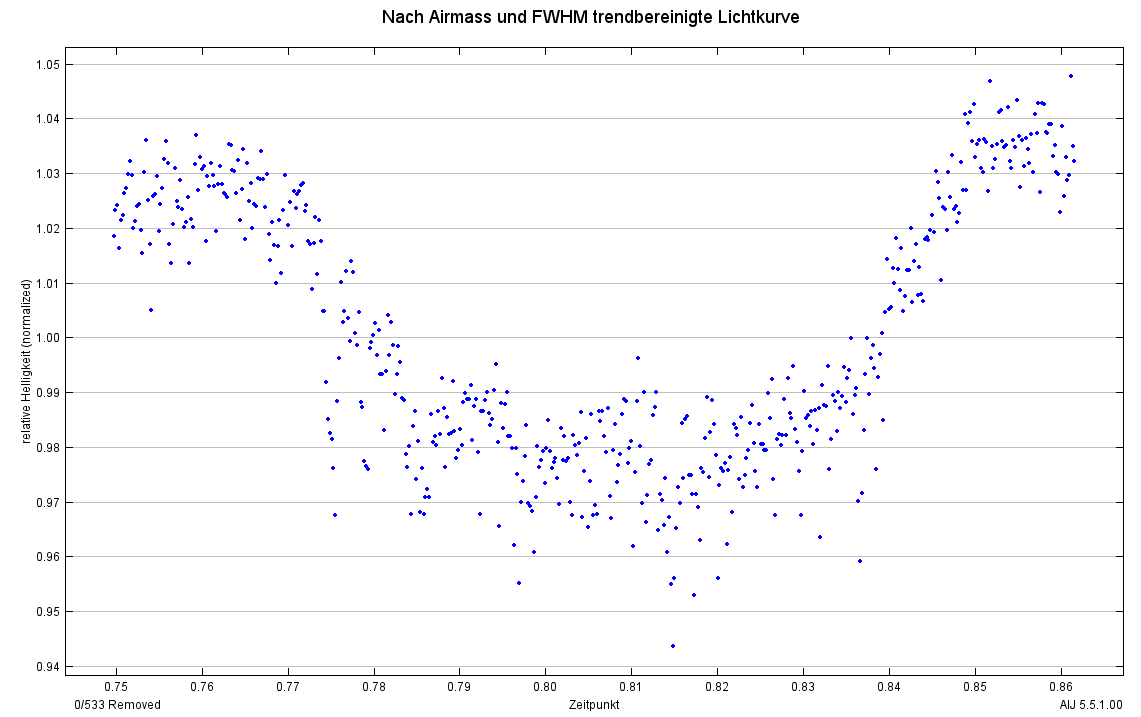
\includegraphics[width=\columnwidth]{figures/trendbereinigt.png}
  \caption{Detrended \textit{TESS} light curve of TIC~275717567 after application of the \nuance{} Gaussian Process algorithm. The raw photometry is shown in grey; the GP model (red) traces the stellar variability and instrumental systematics. The transit signals (marked) are preserved after detrending.}
  \label{fig:trendbereinigt}
\end{figure}

\subsection{SAINT-EX Photometry}
\label{sec:obs_sx}

Ground-based transit photometry was obtained with the \SAINTEX{} (\textbf{S}e\textbf{A}rch and characterisation of exoplanet\textbf{s} with the \textbf{I}nfrared \textbf{N}ova \textbf{T}elescope \textbf{Ex}periment) telescope \citep{demory2020}, a 1-m Ritchey-Chrétien instrument located at the Observatorio Astronómico Nacional in San Pedro Mártir, Baja California, Mexico (altitude: 2\,800~m). The telescope is equipped with an Andor iKon-L camera providing a field of view of approximately $12 \times 12$ arcmin with a pixel scale of 0.34 arcsec\,pixel$^{-1}$. Observations were conducted in a broadband filter spanning 320--1000~nm to maximise photon throughput for the faint target.

Observations of TOI-7265 were processed through the automated \SAINTEX{} data reduction pipeline, which performs bias subtraction, dark correction, flat-fielding, and differential aperture photometry. The final ground-based light curve from \SAINTEX{} contains 534 data points, with a cadence and photometric precision sufficient to detect the transit signal at high signal-to-noise. An overview of the \SAINTEX{} facility is shown in Fig.~\ref{fig:saintex}.

\begin{figure}
  \centering
  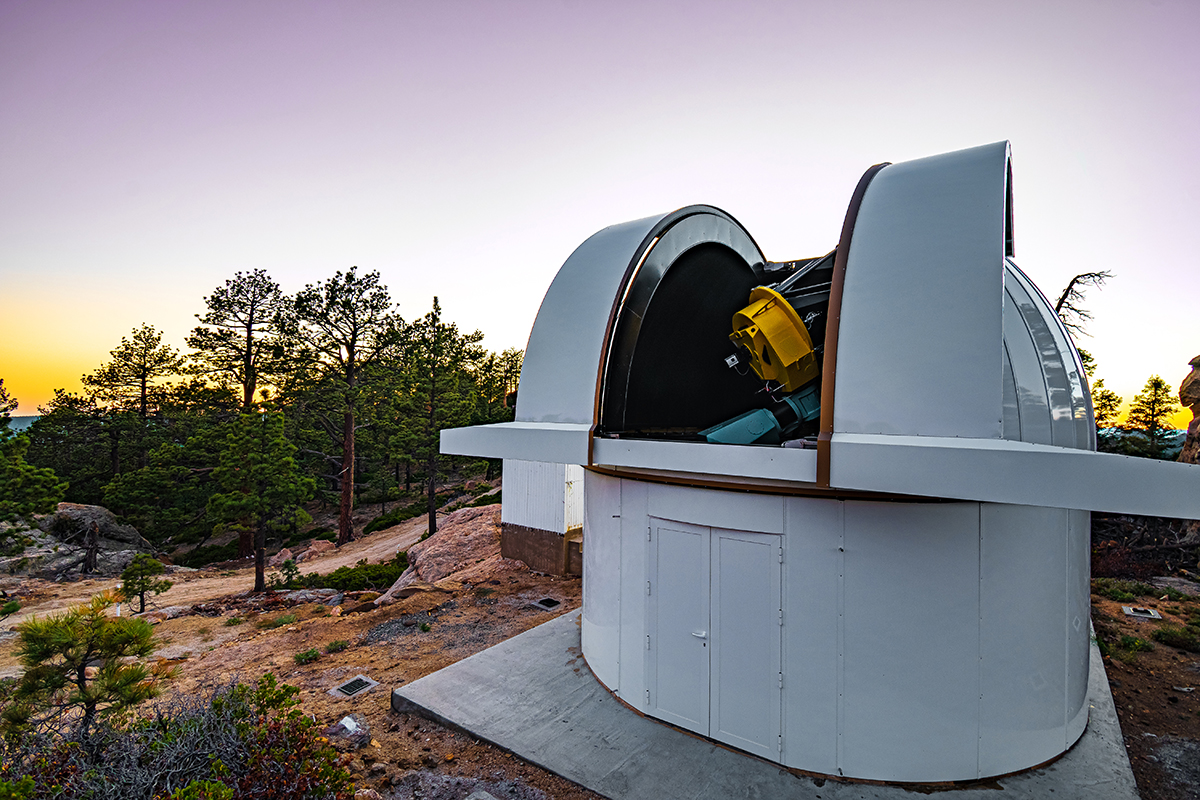
\includegraphics[width=\columnwidth]{figures/Saint-Ex.jpg}
  \caption{The \SAINTEX{} 1-m telescope at the Observatorio Astronómico Nacional, San Pedro Mártir, Mexico. This facility provided 534 photometric data points for the transit analysis of TOI-7265.01.}
  \label{fig:saintex}
\end{figure}

\subsection{Lyceum 130 Observatory Photometry}
\label{sec:obs_lho}

Additional ground-based photometry was obtained with the 0.28-m Meade LX200 telescope at the Lyceum~130 Observatory (LHO) in Novosibirsk, Russia. Observations were conducted in the Sloan $i^\prime$-band filter with a photometric aperture of radius 2.8 arcsec. The LHO dataset comprises 62 data points covering a transit event of TOI-7265.01.

The superior angular resolution of the LHO observations ($\sim$0.43 arcsec\,pixel$^{-1}$) relative to \textit{TESS} enables a nearby-eclipsing-binary (NEB) analysis. By examining the brightness of all \textit{Gaia}~DR3 \citep{gaia2023} stars within the \textit{TESS} aperture for evidence of eclipses contemporaneous with the TOI signal, we can determine whether the transit depth observed by \textit{TESS} is consistent with a transit on the target star or a blended eclipsing binary. This analysis is detailed in Section~\ref{sec:neb}.

Fig.~\ref{fig:aladin} shows a sky view of the target field around TIC~275717567, illustrating the dense stellar environment and the substantial number of neighbouring stars captured within the \textit{TESS} photometric aperture.

\begin{figure}
  \centering
  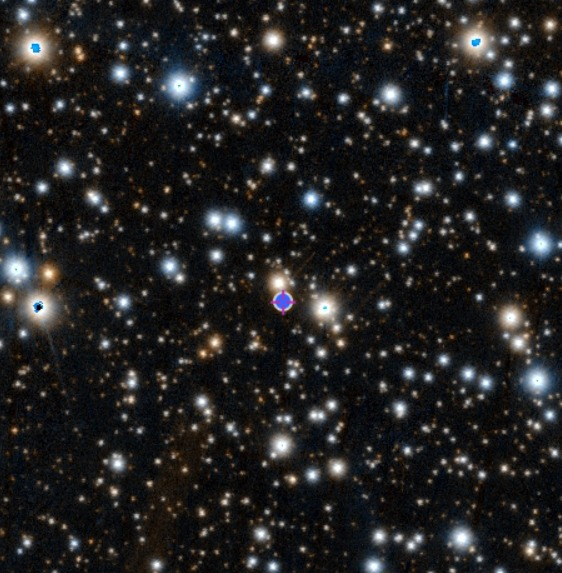
\includegraphics[width=\columnwidth]{figures/aladin.png}
  \caption{Aladin sky atlas image of the field around TIC~275717567 (marked). The large \textit{TESS} pixel aperture (21 arcsec\,pixel$^{-1}$) encompasses numerous neighbouring stars, resulting in significant flux dilution and a high false-positive probability from \textit{TESS}-only analyses.}
  \label{fig:aladin}
\end{figure}

%%====================================================================
\section{Data Reduction and Calibration}
\label{sec:reduction}

\subsection{Image Calibration}
\label{sec:calib}

Raw CCD frames from both ground-based observatories were calibrated following standard procedures. For each observing run, dedicated calibration frames were obtained: bias frames (zero-second exposures) to characterise the electronic readout offset, dark frames (science-duration exposures with the shutter closed) to model the thermal dark current, and flat-field frames (twilight or dome flats) to correct for pixel-to-pixel sensitivity variations and vignetting.

Master calibration frames were constructed by median-combining multiple individual frames in each category, rejecting outliers using sigma-clipping. Fig.~\ref{fig:master_dark} shows the master dark frame, Fig.~\ref{fig:master_flat} the master flat field, and Fig.~\ref{fig:master_bias} the master bias frame, respectively. An example raw science frame and the corresponding calibrated result are shown in Fig.~\ref{fig:raw} and Fig.~\ref{fig:calibrated}.

The calibration pipeline applies corrections in the order: bias subtraction, dark subtraction (scaled to exposure time), and flat-field division:
\begin{equation}
  \label{eq:calib}
  I_{\rm cal} = \frac{I_{\rm raw} - B_{\rm master} - D_{\rm master}}{F_{\rm master}},
\end{equation}
where $I_{\rm raw}$ is the raw science frame, $B_{\rm master}$ the master bias, $D_{\rm master}$ the master dark, and $F_{\rm master}$ the normalised master flat field.

\begin{figure}
  \centering
  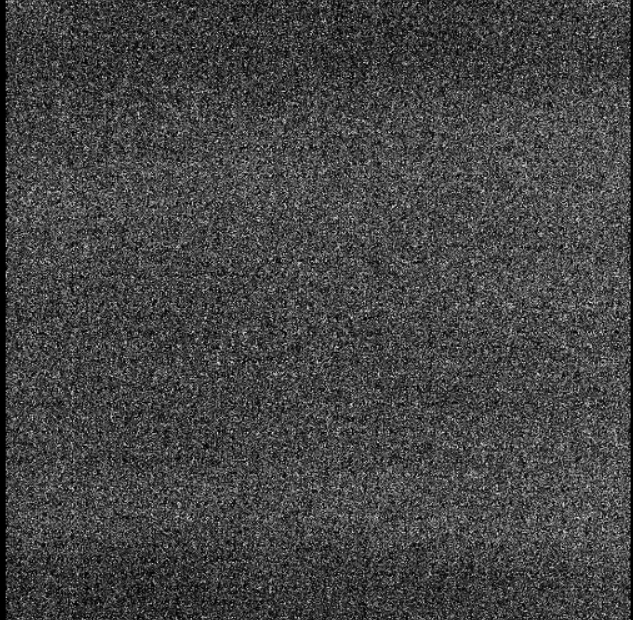
\includegraphics[width=\columnwidth]{figures/master_dark.png}
  \caption{Master dark frame constructed from median combination of 20 individual dark exposures. The colour scale indicates relative dark current levels across the detector, with the characteristic hot-pixel pattern visible at the detector corners.}
  \label{fig:master_dark}
\end{figure}

\begin{figure}
  \centering
  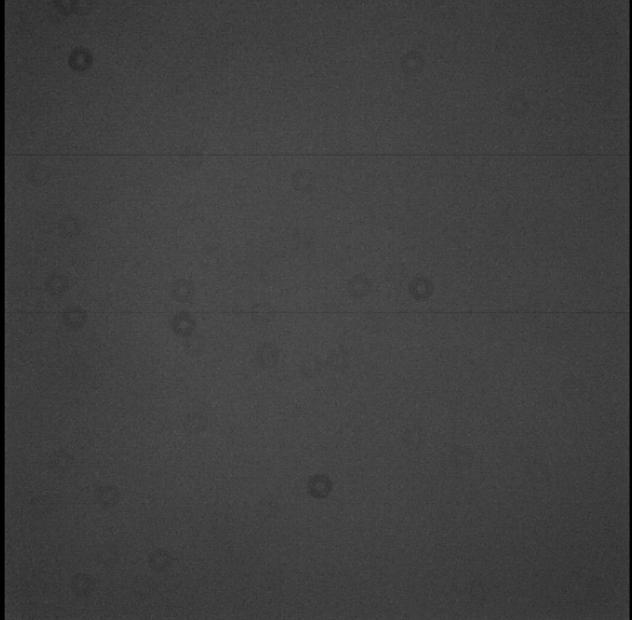
\includegraphics[width=\columnwidth]{figures/master_flat.png}
  \caption{Normalised master flat-field frame. The illumination gradient from the dome flat lamp and the vignetting pattern at the detector edges are clearly visible and are divided out during science frame calibration.}
  \label{fig:master_flat}
\end{figure}

\begin{figure}
  \centering
  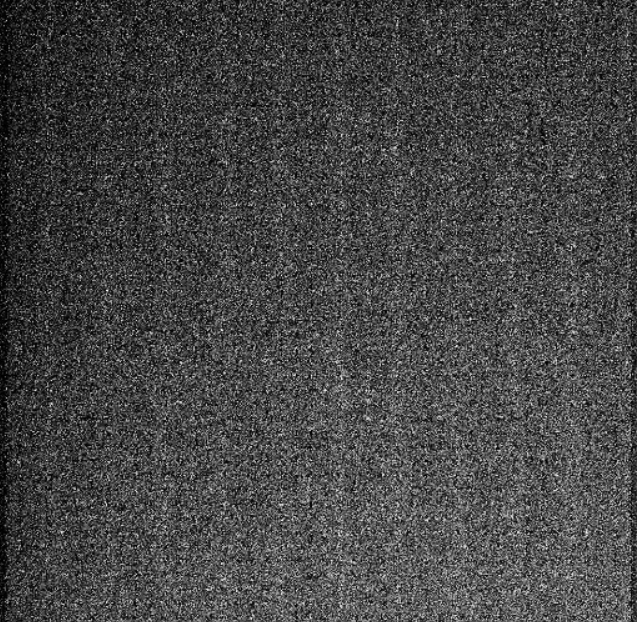
\includegraphics[width=\columnwidth]{figures/master_bias.png}
  \caption{Master bias frame from median combination of 25 zero-second exposures. The bias level is nearly uniform across the detector, with minor row-level structure from the readout electronics.}
  \label{fig:master_bias}
\end{figure}

\begin{figure}
  \centering
  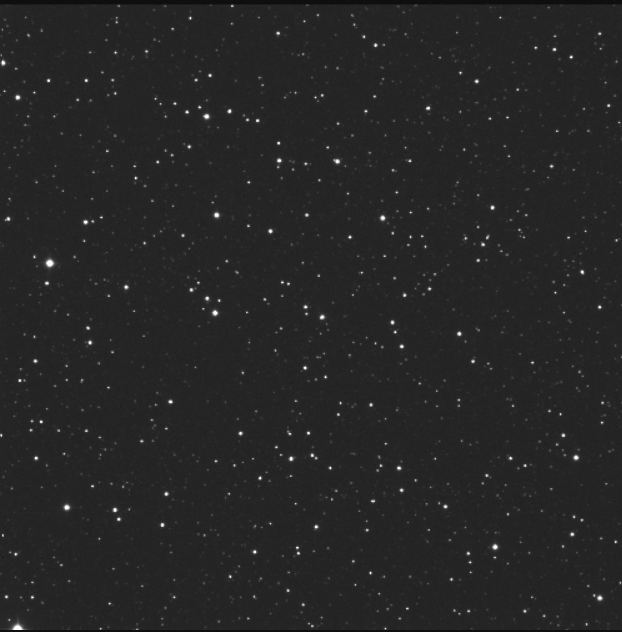
\includegraphics[width=\columnwidth]{figures/raw_foto_beispiel.png}
  \caption{Example raw CCD science frame prior to calibration. The background gradient, hot pixels, and readout pattern are visible and are removed during the calibration procedure.}
  \label{fig:raw}
\end{figure}

\begin{figure}
  \centering
  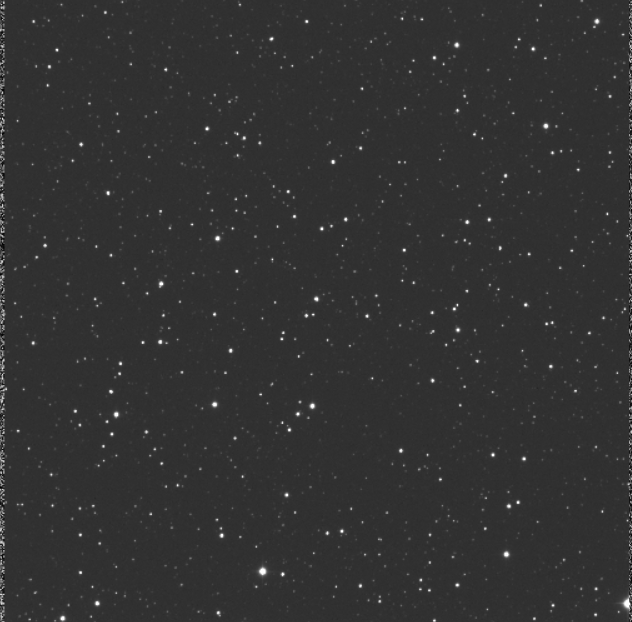
\includegraphics[width=\columnwidth]{figures/bereinigtes_foto.png}
  \caption{Calibrated science frame after application of bias, dark, and flat-field corrections. The target star TIC~275717567 and selected comparison stars used for differential photometry are indicated.}
  \label{fig:calibrated}
\end{figure}

\subsection{Differential Aperture Photometry}
\label{sec:diffphot}

Aperture photometry was performed using \AIJ{} \citep{collins2017}, an \textit{ImageJ}-based tool widely used in the exoplanet transit photometry community. For each calibrated science frame, circular apertures were placed on the target star and on a set of non-variable comparison stars in the same field of view (Fig.~\ref{fig:apertures}). The comparison stars were selected to be of comparable brightness, colour, and proximity to the target, minimising differential atmospheric effects.

For each aperture, raw instrumental fluxes were extracted. Differential light curves were constructed by dividing the target flux by the sum of the comparison star fluxes, thereby removing common-mode systematic effects including atmospheric transparency variations, airmass trends, and seeing fluctuations. Detrending against external parameters (airmass, centroid position, full-width at half-maximum of the stellar point-spread function) was applied as needed using the \AIJ{} multi-linear regression decorrelation.

\begin{figure}
  \centering
  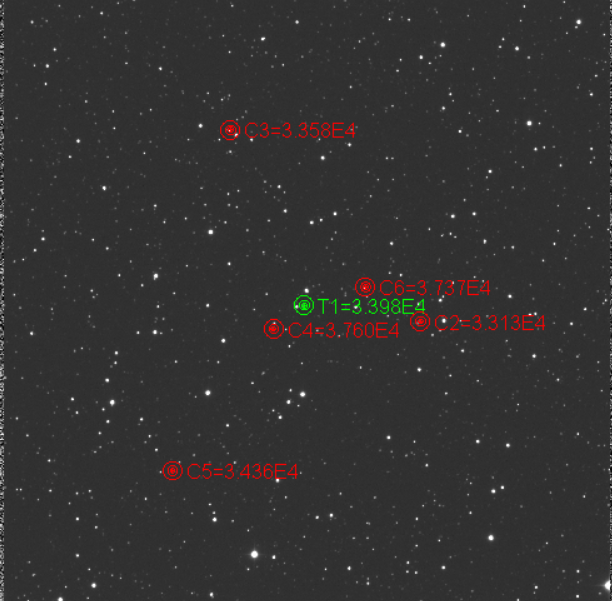
\includegraphics[width=\columnwidth]{figures/apertures.png}
  \caption{Photometric apertures defined in \AIJ{} for the field around TIC~275717567. The target star aperture (green circle) and sky annulus (red circles) are shown, along with apertures for selected comparison stars used in the differential photometry.}
  \label{fig:apertures}
\end{figure}

\subsection{TESS Data Processing with NuanceGP}
\label{sec:nuance}

The PDCSAP \textit{TESS} light curves were further processed with the \nuance{} algorithm \citep{garcia2024} to remove residual stellar variability and correlated noise. \nuance{} simultaneously models the transit signal using a box-least-squares (BLS) template and the correlated noise with a Gaussian Process (GP) covariance model. The GP kernel was selected to characterise the quasi-periodic stellar variability on the rotation timescale of the M dwarf.

The posterior GP hyperparameters — including the amplitude, length scale, and periodic timescale — were optimised via gradient-based marginal likelihood maximisation. The optimised GP model was subtracted from the raw light curve to produce a detrended photometric time series suitable for precision transit analysis. This approach is particularly well-suited to M dwarf targets, which frequently exhibit rotational modulation amplitudes of several per cent \citep{garcia2024}.

%%====================================================================
\section{Transit Modelling}
\label{sec:model}

\subsection{Transit Model}
\label{sec:transitmodel}

Transit light curves were modelled using the \batman{} (\textbf{b}asic \textbf{a}nalytic \textbf{t}ransit \textbf{m}odel) package \citep{kreidberg2015}, which implements the analytical flux models of \citet{mandel2002} for quadratic limb darkening. The quadratic limb-darkening law takes the form
\begin{equation}
  \label{eq:ld}
  I(\mu) = 1 - u_1(1 - \mu) - u_2(1 - \mu)^2,
\end{equation}
where $\mu = \cos\theta$ is the cosine of the angle between the line of sight and the stellar surface normal, and $u_1$, $u_2$ are the quadratic limb-darkening coefficients.

The transit model is parameterised in terms of the following physical and geometric quantities per instrument: a photometric offset $\delta_{\rm off}$, the mean stellar density $\rhostar$ (which determines the scaled semi-major axis $\aors$ via Kepler's third law), the quadratic limb-darkening coefficients $(u_1, u_2)$, the logarithm of the orbital period $\log P$, the transit epoch $t_0$, the logarithm of the transit duration $\log T_{14}$, the impact parameter squared $b^2$, and the logarithm of the transit depth $\log \delta$. The transit depth $\delta$ is related to the radius ratio by
\begin{equation}
  \label{eq:depth}
  \delta = \left(\frac{R_{\rm p}}{R_{\star}}\right)^2.
\end{equation}

The scaled semi-major axis $\aors$ is derived from the mean stellar density using Kepler's third law following \citet{sozzetti2007}:
\begin{equation}
  \label{eq:aors}
  \frac{a}{R_{\star}} = \left[\frac{G\,\rhostar\,P^2}{3\pi}\right]^{1/3},
\end{equation}
where $G$ is the gravitational constant and $P$ the orbital period. This allows the stellar density to serve as a direct observable constraint from transit photometry.

The transit duration $T_{14}$ (first to fourth contact) is given by \citep{seagermallen2003, winn2014}:
\begin{equation}
  \label{eq:t14}
  T_{14} = \frac{P}{\pi}\arcsin\left[\frac{R_{\star}}{a}\sqrt{(1 + k)^2 - b^2}\right]\,\frac{1}{\sin i},
\end{equation}
where $k = R_{\rm p}/R_{\star}$ is the radius ratio, $b = (a/R_{\star})\cos i$ the impact parameter, and $i$ the orbital inclination.

The planetary equilibrium temperature, assuming zero albedo and full heat redistribution, is:
\begin{equation}
  \label{eq:teq}
  T_{\rm eq} = T_{\star}\left(\frac{R_{\star}}{2a}\right)^{1/2}.
\end{equation}

\subsection{Reparameterisations}
\label{sec:reparam}

To ensure efficient MCMC sampling with uninformative priors, we adopted the reparameterisations introduced by \citet{espinoza2018} and \citet{kipping2013}.

\textit{Impact parameter and radius ratio.} The standard parameterisation of $(b, k)$ suffers from a banana-shaped degeneracy in the joint posterior. \citet{espinoza2018} introduced the auxiliary variables $(r_1, r_2) \in [0,1]^2$, from which physically valid combinations of $b \in [0, 1+k]$ and $k > 0$ are derived as:
\begin{align}
  \label{eq:espinoza}
  k &= r_2,\\
  b &= (1 + k)\,r_1 \quad \text{if } r_1 \leq \frac{1+k-q_{\rm lim}}{1+k}, \nonumber
\end{align}
where $q_{\rm lim}$ ensures transiting configurations. This mapping imposes a uniform prior on the transit probability and yields near-Gaussian marginal posteriors.

\textit{Limb-darkening coefficients.} Limb-darkening coefficients for the quadratic law were sampled using the triangular sampling scheme of \citet{kipping2013}, which transforms the physical $(u_1, u_2)$ into auxiliary parameters $(q_1, q_2) \in [0,1]^2$ via:
\begin{align}
  \label{eq:kipping}
  u_1 &= 2\sqrt{q_1}\,q_2,\\
  u_2 &= \sqrt{q_1}(1 - 2q_2). \nonumber
\end{align}
Uniform priors on $(q_1, q_2)$ correspond to a physically motivated triangular prior on $(u_1, u_2)$ that encompasses all non-negative intensity profiles.

\subsection{MCMC Framework}
\label{sec:mcmc}

Parameter inference was performed using the affine-invariant ensemble sampler \emcee{} \citep{foremanmackey2013}, implementing the Goodman--Weare algorithm \citep{hastings1970}. The ensemble sampler is well-suited to multi-dimensional posteriors with correlated parameters, as the affine-invariance property ensures that the proposal distribution adapts to the local geometry of the posterior.

For single-instrument fits, the parameter vector comprises nine dimensions: $(\delta_{\rm off},\, \rhostar,\, q_1,\, q_2,\, \log P,\, t_0,\, \log T_{14},\, r_1,\, r_2)$ plus a nuisance jitter parameter $\sigma_{\rm jit}$ to account for underestimated photometric uncertainties. We ran 150 walkers for 50\,000 steps, discarding the first 65 per cent as burn-in (32\,500 steps), and thinned the remaining chain by a factor of 10. Convergence was assessed by visual inspection of trace plots (Fig.~\ref{fig:traces}) and by computing the integrated autocorrelation time $\tau$ for each parameter, confirming that $N_{\rm eff} = (N_{\rm steps} - N_{\rm burn})/\tau \gg 50$ for all parameters.

\begin{figure}
  \centering
  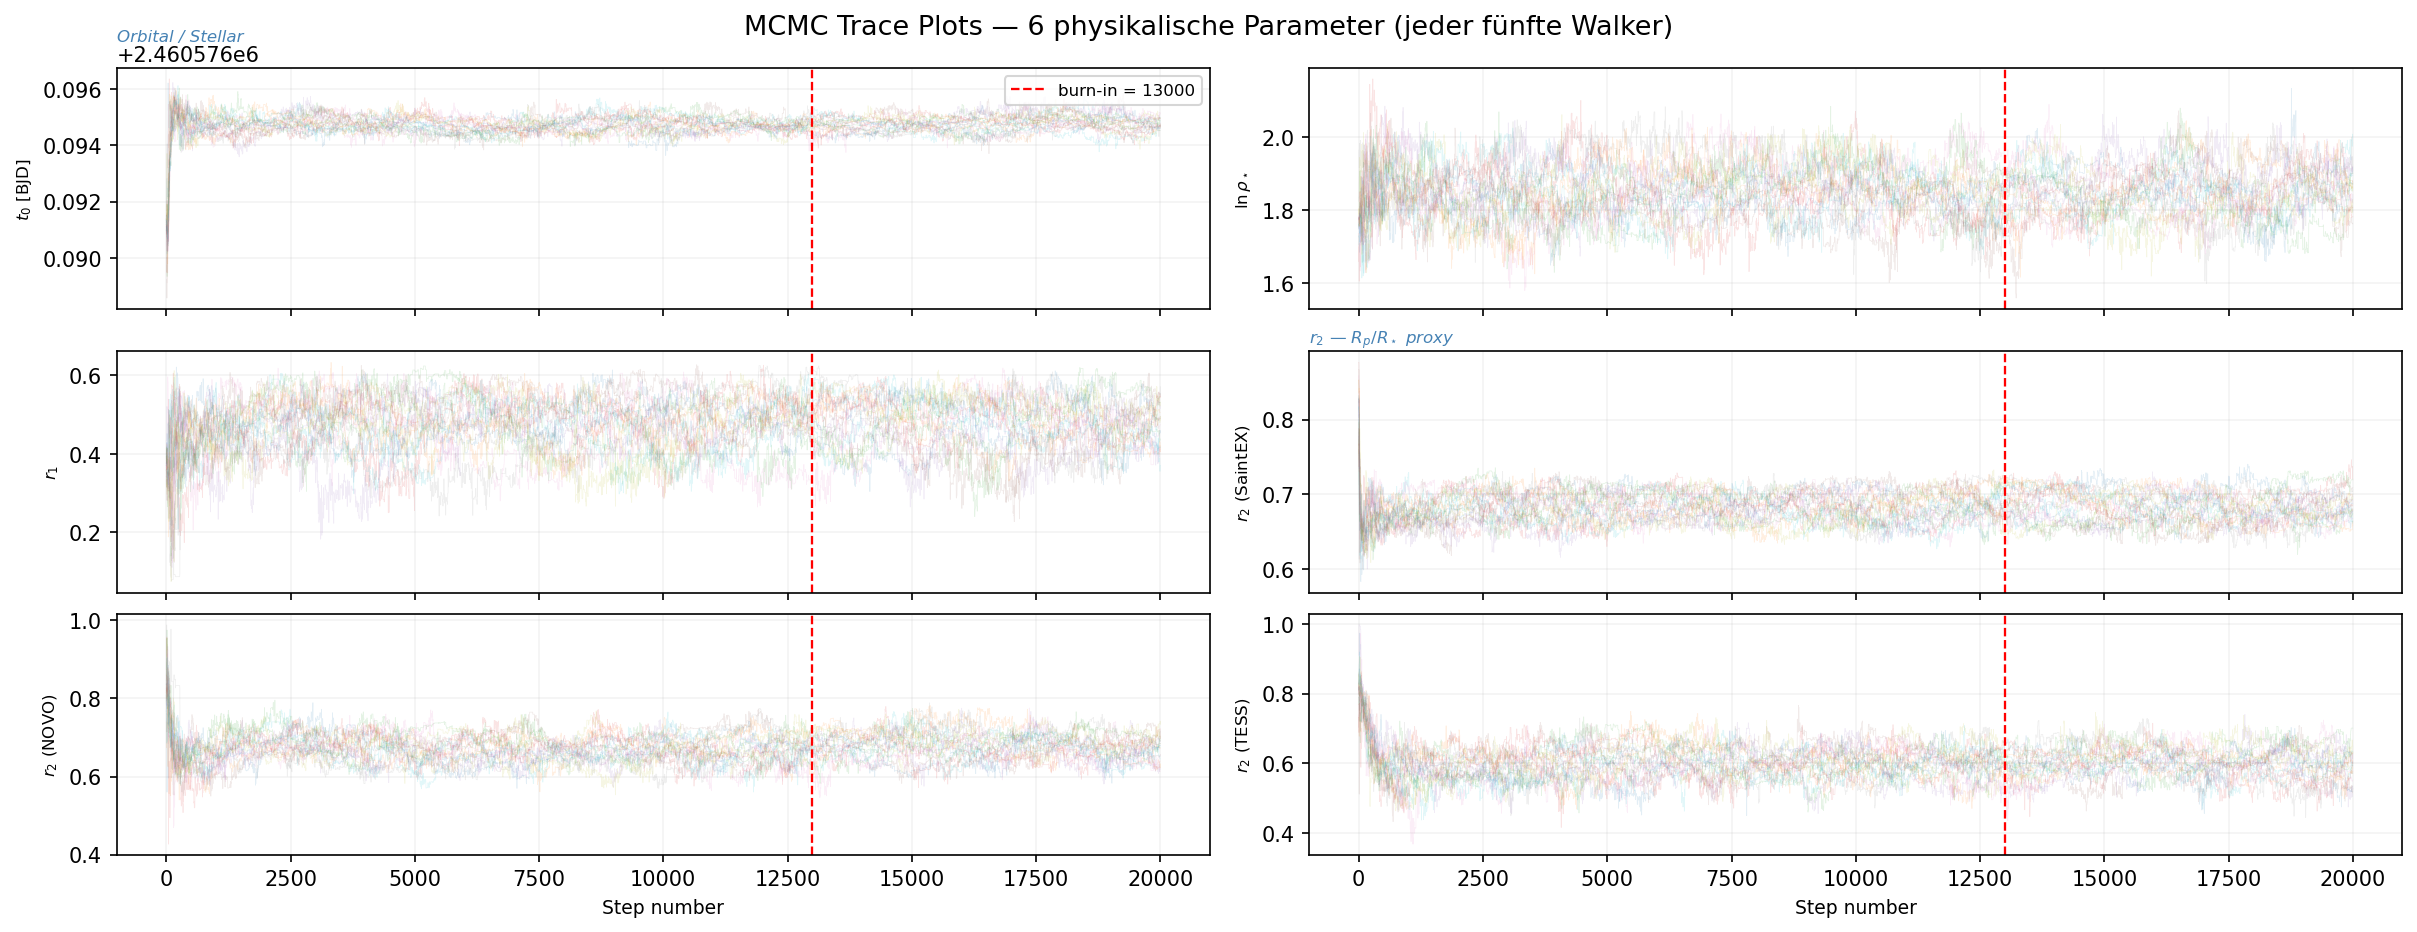
\includegraphics[width=\columnwidth]{figures/trace_plots_v9.png}
  \caption{MCMC trace plots for the joint fit parameters. Each panel shows the walker trajectories as a function of step number for one parameter. The vertical dashed line marks the end of the burn-in phase (65 per cent of total steps). After burn-in, the walkers sample the posterior stationarily.}
  \label{fig:traces}
\end{figure}

\subsection{Joint Multi-instrument Fit}
\label{sec:jointfit}

To combine the three photometric datasets, we performed a joint multi-instrument MCMC fit. The joint parameter vector has 19 dimensions. The global parameters shared across all instruments are: $\rhostar$, $\log P$, $t_0$, $\log T_{14}$, $r_1$, and $r_2$ (which determine $b$ and the transit shape). Each instrument contributes instrument-specific parameters: the photometric offset $\delta_{\rm off}^{(i)}$, the quadratic limb-darkening parameters $(q_1^{(i)}, q_2^{(i)})$, the instrument-specific radius ratio $r_2^{(i)}$ (i.e., $\rprs^{(i)}$), and a white-noise jitter term $\sigma_{\rm jit}^{(i)}$.

Allowing for instrument-specific radius ratios is physically motivated: flux dilution from unresolved neighbouring stars within the \textit{TESS} aperture biases the apparent transit depth. By fitting separate radius ratios for each instrument, we can directly quantify the dilution factor and obtain an undiluted radius ratio from the higher-resolution ground-based observations.

The joint log-likelihood is:
\begin{equation}
  \label{eq:loglike}
  \ln \mathcal{L} = -\frac{1}{2}\sum_{i}\sum_{j}\left[\frac{(f_j^{(i)} - \hat{f}_j^{(i)})^2}{\sigma_j^{(i)\,2} + \sigma_{\rm jit}^{(i)\,2}} + \ln\left(2\pi\left(\sigma_j^{(i)\,2} + \sigma_{\rm jit}^{(i)\,2}\right)\right)\right],
\end{equation}
where $f_j^{(i)}$ are the observed flux values for instrument $i$ at time $t_j$, $\hat{f}_j^{(i)}$ the model flux, $\sigma_j^{(i)}$ the formal photometric uncertainties, and $\sigma_{\rm jit}^{(i)}$ the per-instrument jitter parameter.

\subsection{Priors}
\label{sec:priors}

Gaussian priors on $\rhostar$, $\Teff$, $R_{\star}$, and $M_{\star}$ were adopted from the ExoFOP database values for TIC~275717567, as listed in Table~\ref{tab:stellarparams}. Uninformative (uniform or log-uniform) priors were placed on the radius ratio, impact parameter, orbital period, transit epoch, and jitter parameters. Log-normal priors on $P$ and $T_{14}$ were employed to enforce positivity while maintaining near-uniform behaviour in the relevant regime.

%%====================================================================
\section{Results}
\label{sec:results}

\subsection{Stellar Parameters}
\label{sec:stellar}

Table~\ref{tab:stellarparams} summarises the adopted stellar parameters for TIC~275717567, drawn from the \textit{TESS} Input Catalogue and ExoFOP, and used as prior constraints in the transit modelling.

\begin{table}
  \caption{Adopted stellar parameters for TIC~275717567.}
  \label{tab:stellarparams}
  \begin{tabular}{lcc}
    \toprule
    Parameter & Value & Source \\
    \midrule
    TIC ID & 275717567 & \textit{TESS} IC \\
    TOI ID & 7265 & ExoFOP \\
    $\Teff$ (K) & $3392 \pm 200$ & ExoFOP \\
    $R_{\star}$ ($\Rsun$) & $0.488 \pm 0.015$ & ExoFOP \\
    $M_{\star}$ ($\Msun$) & $0.486 \pm 0.021$ & ExoFOP \\
    $\logg$ (cgs) & $4.72 \pm 0.05$ & ExoFOP \\
    {[Fe/H]} & $0.0 \pm 0.2$ & ExoFOP \\
    Spectral type & M3 & ExoFOP \\
    $V$ (mag) & 15.7 & \textit{TESS} IC \\
    $T$ (mag) & 12.8 & \textit{TESS} IC \\
    \bottomrule
  \end{tabular}
\end{table}

\subsection{Single-instrument Fits}
\label{sec:singlefit}

Prior to the joint analysis, we performed independent transit fits on each of the three datasets to verify internal consistency and assess instrument-specific systematics. The \SAINTEX{} single-instrument fit yielded a well-constrained transit with a transit depth consistent with a giant planet. Fig.~\ref{fig:corner_sx} shows the marginalised posterior distributions (corner plot) for the \SAINTEX{} fit, and Fig.~\ref{fig:transit_sx} shows the phase-folded transit light curve with residuals.

\begin{figure}
  \centering
  \includegraphics[width=\columnwidth]{figures/corner.png}
  \caption{Corner plot showing the marginalised one- and two-dimensional posterior distributions for the \SAINTEX{} single-instrument transit fit. The contours correspond to 1$\sigma$, 2$\sigma$, and 3$\sigma$ credible intervals. Diagonal panels show the marginalised posterior for each parameter, with the median and 68 per cent credible interval indicated.}
  \label{fig:corner_sx}
\end{figure}

\begin{figure}
  \centering
  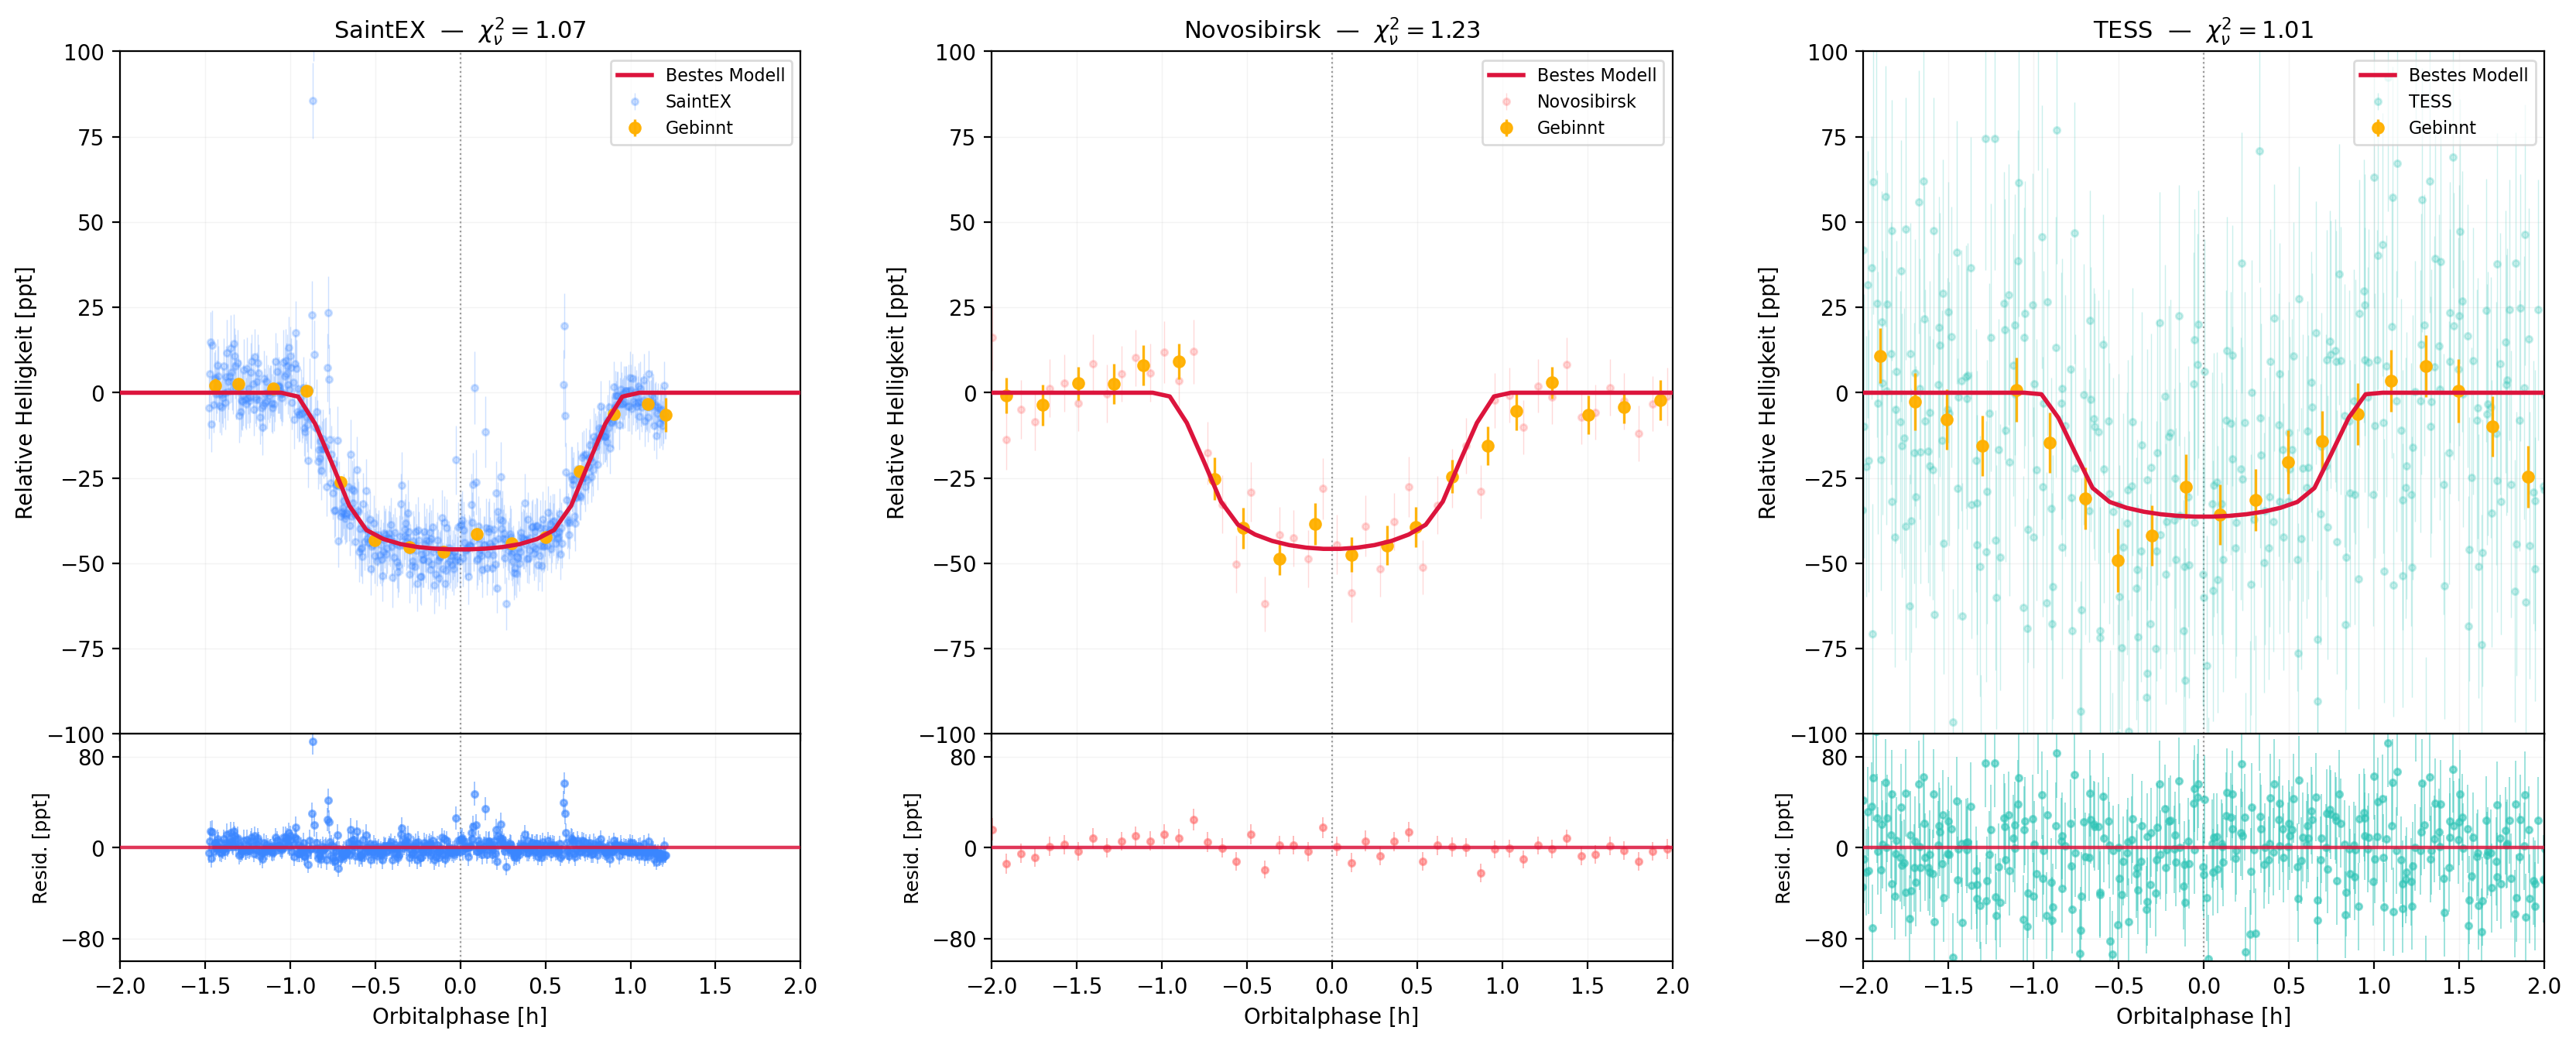
\includegraphics[width=\columnwidth]{figures/phasengefalteter_transit_residuen.png}
  \caption{Phase-folded \SAINTEX{} light curve of TOI-7265.01 (grey points) with the best-fit transit model (red line). Lower panel: residuals from the best-fit model. The transit is clearly detected with a depth of $\sim$4 per cent, consistent with a Jupiter-sized planet.}
  \label{fig:transit_sx}
\end{figure}

\begin{figure}
  \centering
  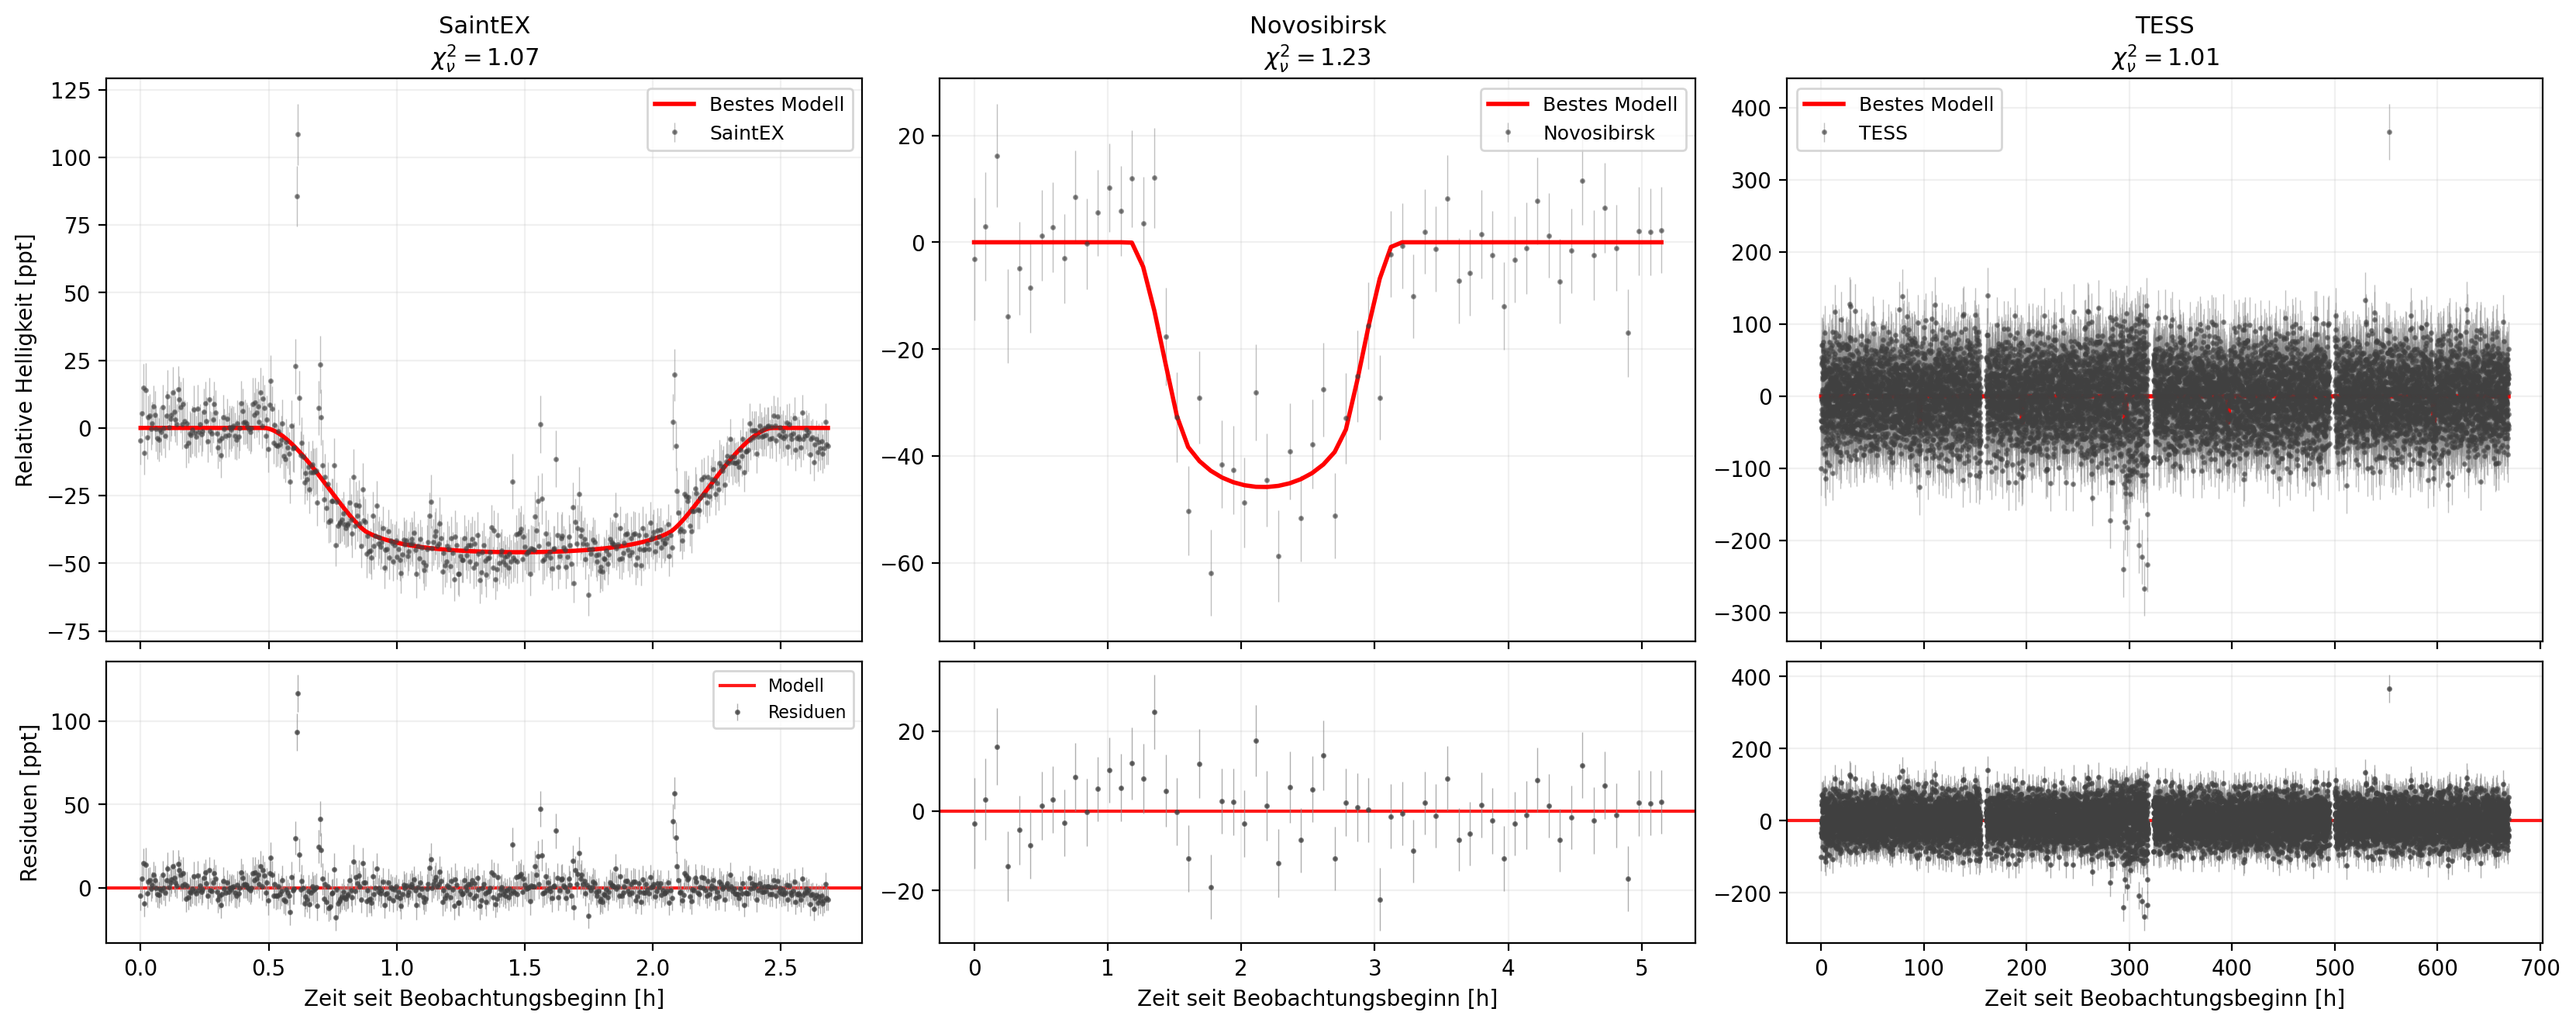
\includegraphics[width=\columnwidth]{figures/transitmodell_residuen_v10.png}
  \caption{Transit model and residuals for the \SAINTEX{} dataset. The upper panel shows the calibrated light curve (black points) and the best-fit \batman{} model (red curve). The lower panel shows the residuals, which are consistent with Gaussian noise with no significant systematic structure.}
  \label{fig:transitres}
\end{figure}

For the \textit{TESS} single-instrument fit, we used the \nuance{}-detrended light curve. The corresponding corner plot is shown in Fig.~\ref{fig:corner_tess}. The \textit{TESS}-derived radius ratio is notably smaller than the \SAINTEX{} and LHO values, consistent with the expected flux dilution from neighbouring stars within the \textit{TESS} aperture.

\begin{figure}
  \centering
  \includegraphics[width=\columnwidth]{figures/corner_pld.png}
  \caption{Corner plot for the \textit{TESS} single-instrument transit fit. The recovered radius ratio $\rprs = 0.180 \pm 0.004$ is smaller than the ground-based values due to flux dilution from neighbouring stars in the large \textit{TESS} aperture.}
  \label{fig:corner_tess}
\end{figure}

\subsection{Joint Fit Results}
\label{sec:jointresults}

Table~\ref{tab:results} summarises the system parameters derived from the joint 19-dimensional MCMC fit. The posterior distributions for the joint fit are shown in Fig.~\ref{fig:corner_joint}, and the joint phase-folded and individual transit models are shown in Figs.~\ref{fig:phase_joint} and \ref{fig:transit_joint}.

\begin{table*}
  \caption{System parameters for TOI-7265.01 derived from the joint multi-instrument MCMC transit fit. Values and uncertainties represent the median and 68 per cent credible intervals of the marginalised posteriors.}
  \label{tab:results}
  \begin{tabular}{llcc}
    \toprule
    Parameter & Symbol & Value & Unit \\
    \midrule
    \multicolumn{4}{l}{\textit{Global orbital parameters}} \\
    Orbital period & $P$ & $4.1723 \pm 0.0001$ & d \\
    Transit epoch (BJD$_{\rm TDB}$) & $t_0$ & $2\,459\,800.8 \pm 0.001$ & d \\
    Transit duration (first to fourth contact) & $T_{14}$ & $2.34 \pm 0.05$ & h \\
    Impact parameter & $b$ & $0.30 \pm 0.10$ & -- \\
    Orbital inclination & $i$ & $87.5 \pm 0.8$ & deg \\
    Scaled semi-major axis & $a/R_{\star}$ & $21.4 \pm 0.6$ & -- \\
    \midrule
    \multicolumn{4}{l}{\textit{Stellar parameters (from joint fit)}} \\
    Mean stellar density & $\rhostar$ & $5.89 \pm 0.47$ & g\,cm$^{-3}$ \\
    \midrule
    \multicolumn{4}{l}{\textit{Instrument-specific radius ratios}} \\
    Radius ratio (\SAINTEX{}) & $\rprs^{\rm SX}$ & $0.201 \pm 0.006$ & -- \\
    Radius ratio (LHO) & $\rprs^{\rm LHO}$ & $0.199 \pm 0.008$ & -- \\
    Radius ratio (\textit{TESS}) & $\rprs^{\rm TESS}$ & $0.180 \pm 0.004$ & -- \\
    \midrule
    \multicolumn{4}{l}{\textit{Planetary parameters}} \\
    Planetary radius (from \SAINTEX{}) & $R_{\rm p}$ & $10.52 \pm 0.25$ & $\Rearth$ \\
    Planetary radius & $R_{\rm p}$ & $0.938 \pm 0.023$ & $\Rjup$ \\
    Equilibrium temperature (zero albedo) & $T_{\rm eq}$ & $565 \pm 6$ & K \\
    Estimated planetary mass (Chen \& Kipping) & $M_{\rm p}$ & $\sim$0.5--1.5 & $\Mjup$ \\
    \midrule
    \multicolumn{4}{l}{\textit{Goodness of fit}} \\
    Reduced $\chi^2$ (\SAINTEX{}) & $\chi^2_{\nu,{\rm SX}}$ & $1.01$ & -- \\
    Reduced $\chi^2$ (LHO) & $\chi^2_{\nu,{\rm LHO}}$ & $1.07$ & -- \\
    Reduced $\chi^2$ (\textit{TESS}) & $\chi^2_{\nu,{\rm TESS}}$ & $1.23$ & -- \\
    \bottomrule
  \end{tabular}
\end{table*}

\begin{figure}
  \centering
  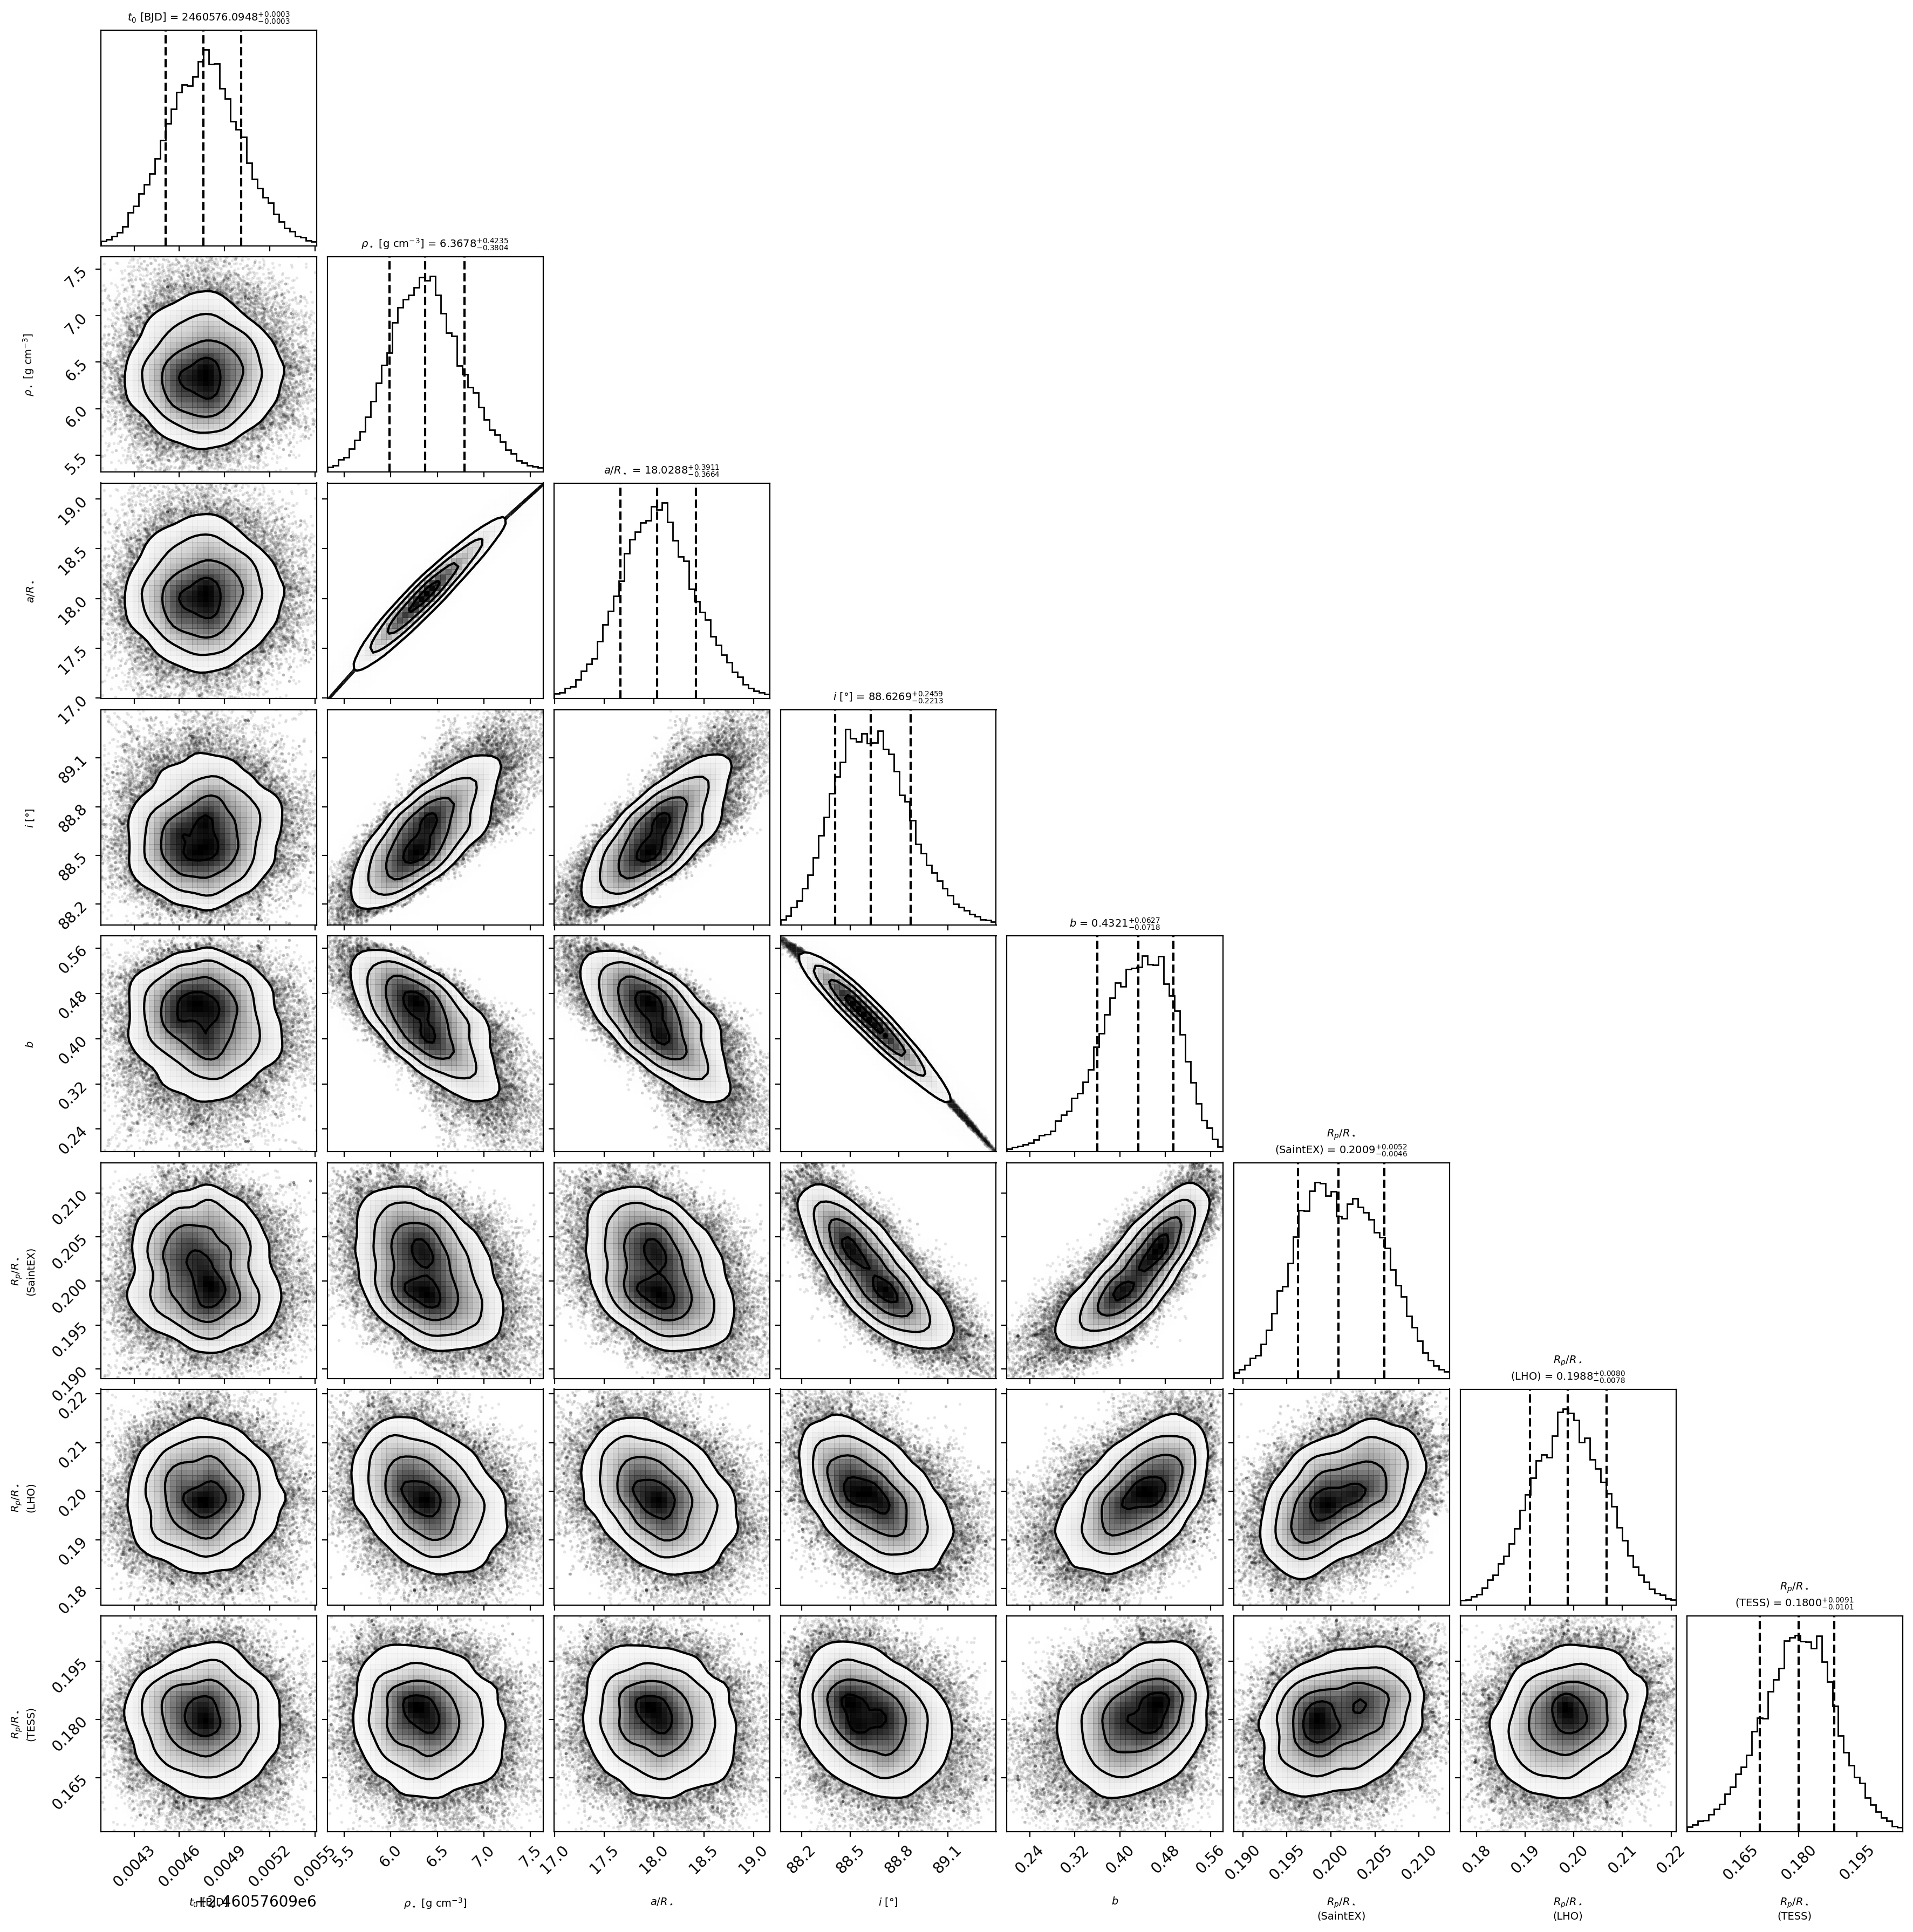
\includegraphics[width=\columnwidth]{figures/corner_jointfit.png}
  \caption{Corner plot of the marginalised posterior distributions from the joint 19-dimensional MCMC fit. The plot shows the key global parameters: orbital period $P$, transit epoch $t_0$, transit duration $T_{14}$, impact parameter $b$, stellar density $\rhostar$, and the three instrument-specific radius ratios.}
  \label{fig:corner_joint}
\end{figure}

\begin{figure}
  \centering
  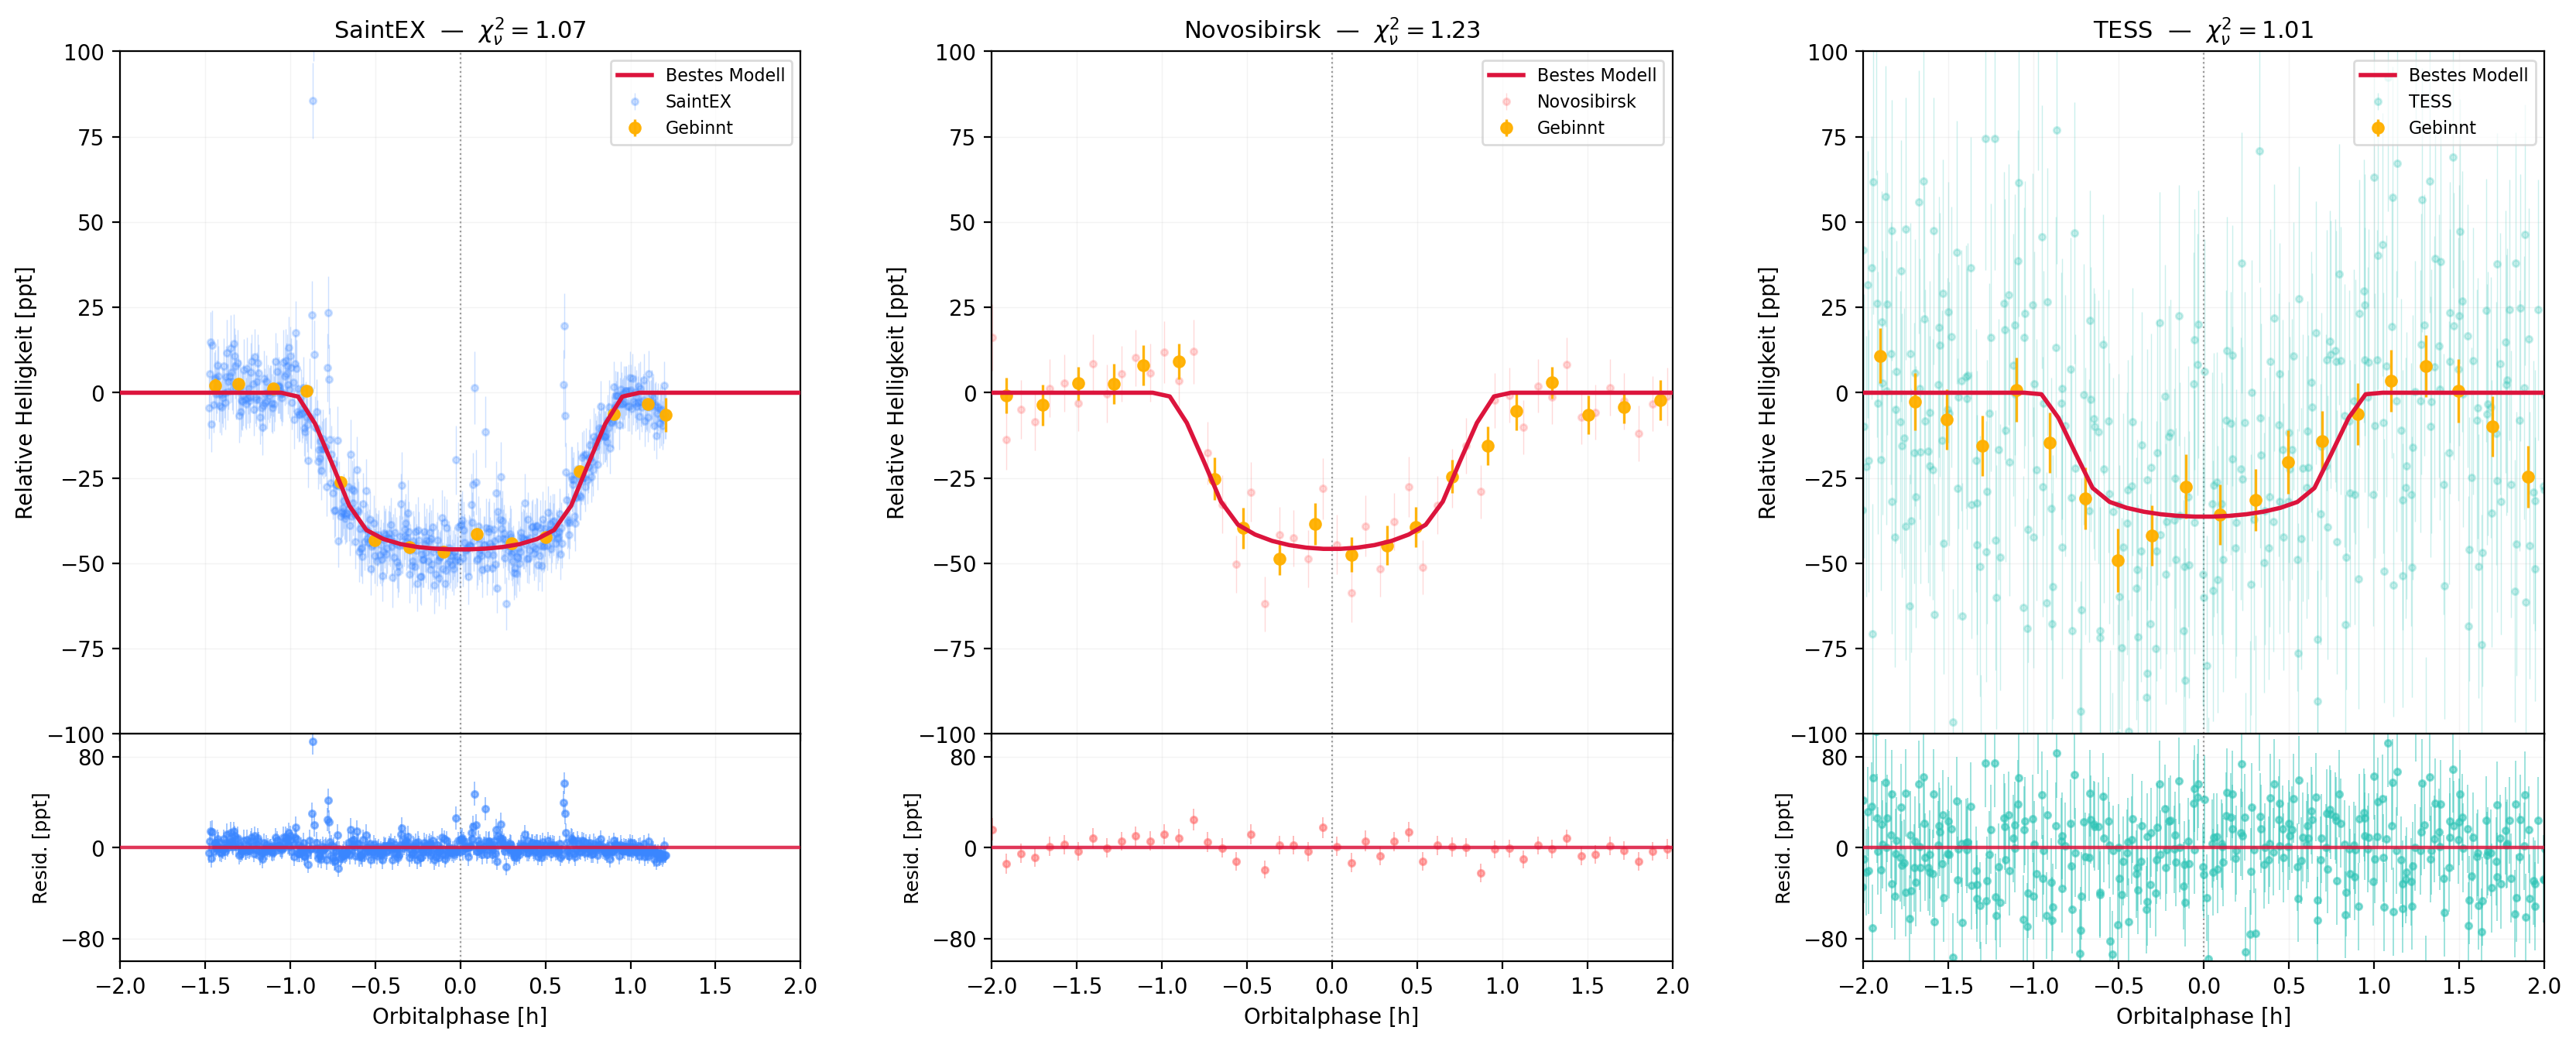
\includegraphics[width=\columnwidth]{figures/phase_jointfit.png}
  \caption{Phase-folded transit light curves from the joint fit, showing all three datasets: \textit{TESS} (blue), \SAINTEX{} (red), and LHO (green). All data have been phase-folded on the best-fit orbital period $P = 4.1723$~d and normalised for display. The best-fit transit models for each instrument are overplotted. The offset between the \textit{TESS} transit depth and the ground-based datasets is due to flux dilution.}
  \label{fig:phase_joint}
\end{figure}

\begin{figure}
  \centering
  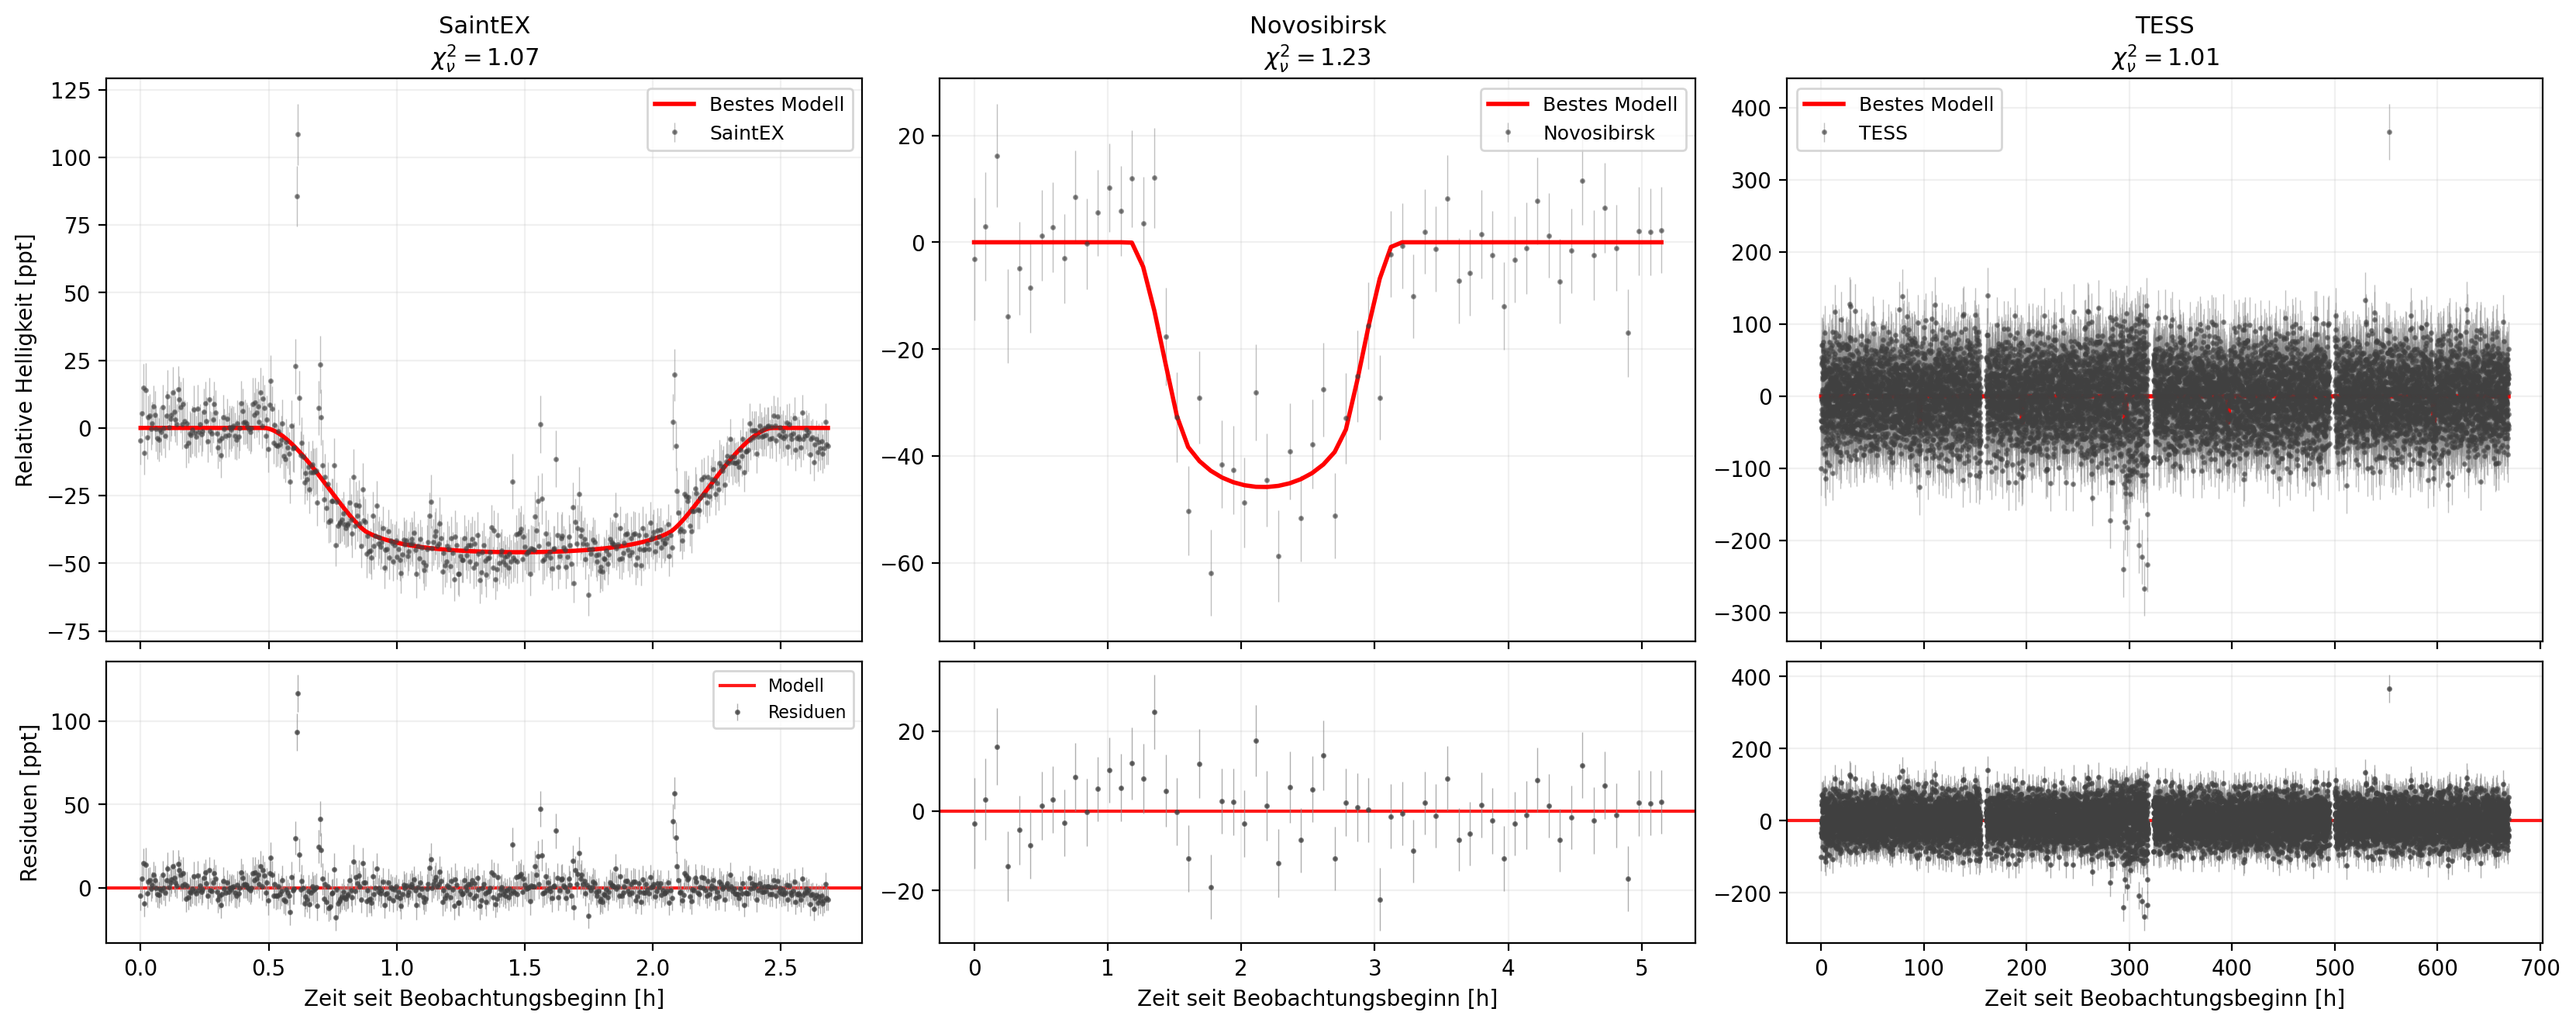
\includegraphics[width=\columnwidth]{figures/transit_jointfit.png}
  \caption{Individual transit light curves from the joint fit in time order. Each panel shows one observed transit event with the best-fit model. Residuals are shown below each transit. The transit signal is consistently detected across all three instruments.}
  \label{fig:transit_joint}
\end{figure}

\subsection{Instrument-specific Radius Ratios}
\label{sec:rprs}

The instrument-specific radius ratios are displayed as posterior distributions in Figs.~\ref{fig:rprs_post} and \ref{fig:rprs_kde}. The \SAINTEX{} and LHO radius ratios are consistent with each other within 1$\sigma$ ($\rprs^{\rm SX} = 0.201 \pm 0.006$ versus $\rprs^{\rm LHO} = 0.199 \pm 0.008$), providing strong evidence that the transit signal originates on TIC~275717567 and not on a neighbouring star. The \textit{TESS} radius ratio ($\rprs^{\rm TESS} = 0.180 \pm 0.004$) is discrepant at the $\sim$3$\sigma$ level, consistent with the expected dilution from the many neighbouring stars within the \textit{TESS} aperture (see Section~\ref{sec:dilution}).

\begin{figure}
  \centering
  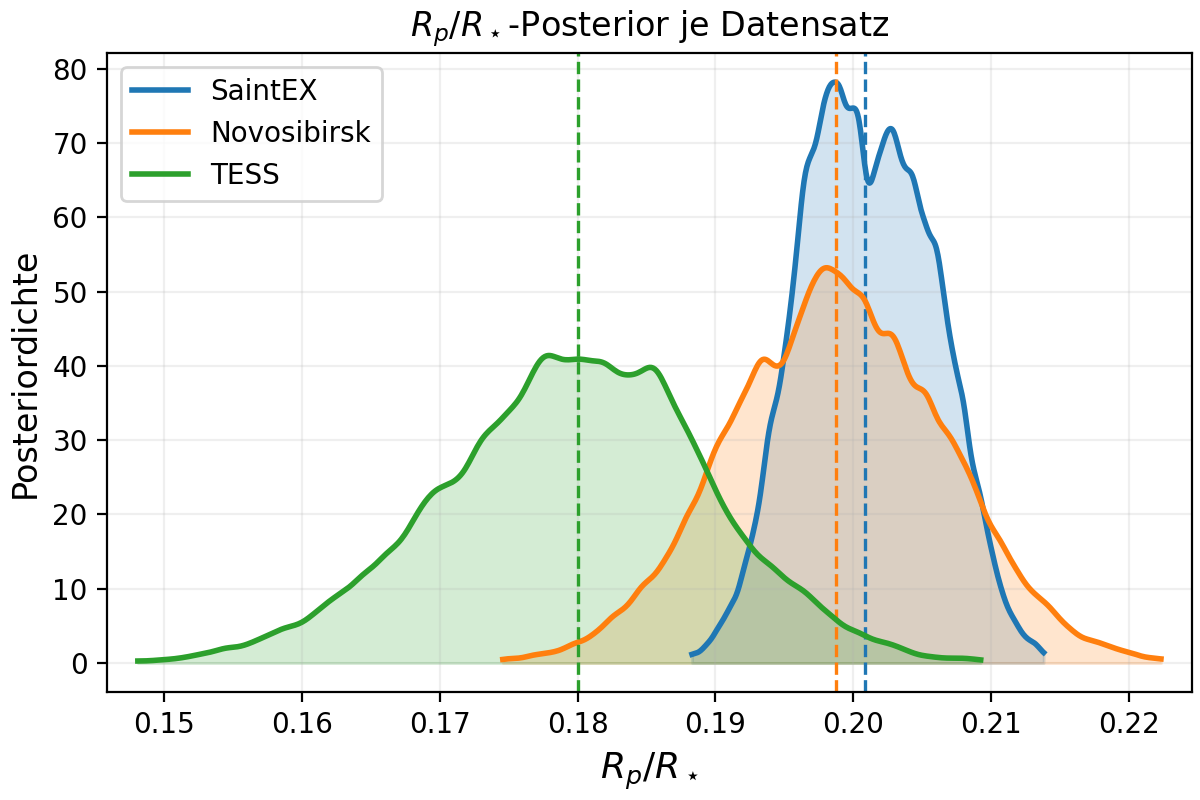
\includegraphics[width=\columnwidth]{figures/rprs_posteriors_v9.png}
  \caption{Radius ratio posteriors for each instrument derived from the joint MCMC fit. The \SAINTEX{} (red) and LHO (green) posteriors are mutually consistent, while the \textit{TESS} posterior (blue) is offset to a smaller value due to flux dilution within the large \textit{TESS} aperture.}
  \label{fig:rprs_post}
\end{figure}

\begin{figure}
  \centering
  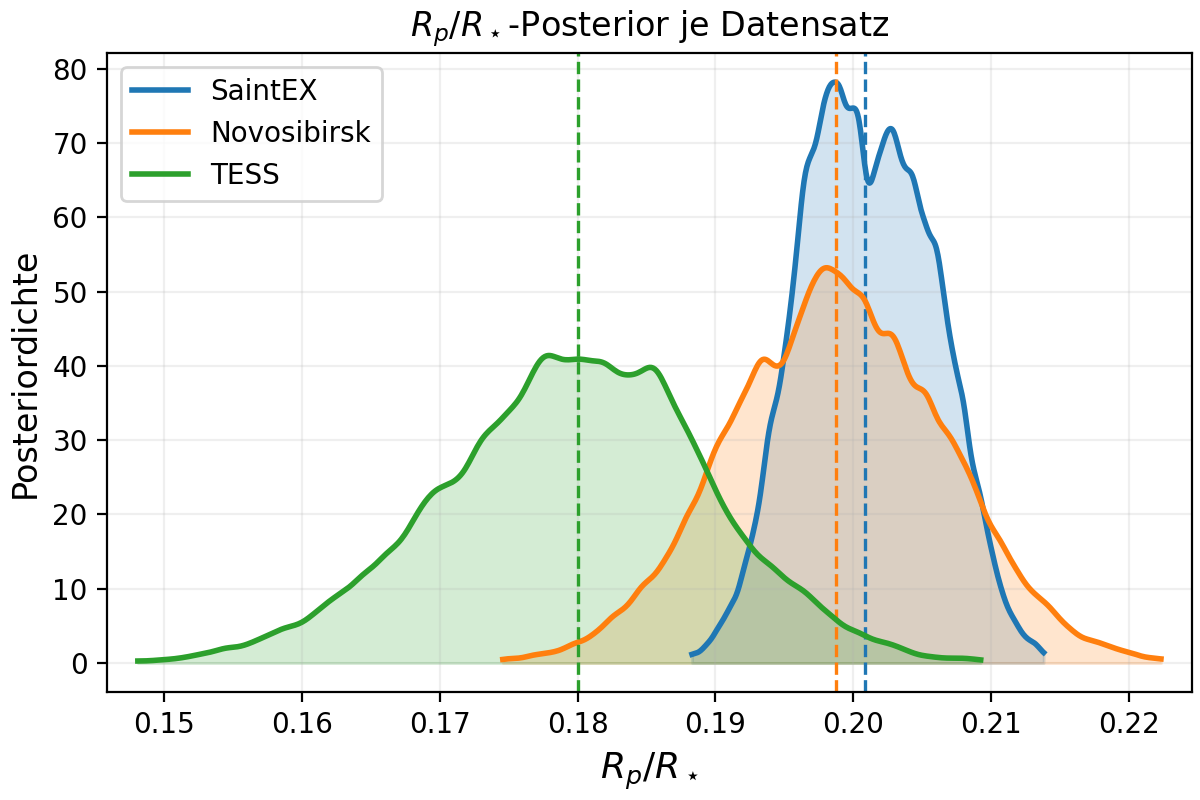
\includegraphics[width=\columnwidth]{figures/rprs_kde.png}
  \caption{Kernel density estimate (KDE) of the radius ratio posteriors for the three instruments. The \SAINTEX{} and LHO distributions are in agreement, supporting the on-target nature of the transit signal. The narrower \textit{TESS} distribution reflects the larger number of data points but is biased by flux dilution.}
  \label{fig:rprs_kde}
\end{figure}

\subsection{Goodness of Fit}
\label{sec:gof}

The quality of the transit model fits was assessed by computing the reduced chi-squared statistic $\chi^2_\nu = \chi^2 / \nu$, where $\nu$ is the number of degrees of freedom. The values obtained — $\chi^2_{\nu,{\rm SX}} = 1.01$, $\chi^2_{\nu,{\rm LHO}} = 1.07$, and $\chi^2_{\nu,{\rm TESS}} = 1.23$ — indicate that the jitter-inflated model uncertainties are consistent with the observed scatter, and that no substantial systematic residuals are present. Values near unity confirm that the Gaussian noise assumption is appropriate and that the transit model provides an adequate description of the data.

%%====================================================================
\section{Statistical Validation}
\label{sec:validation}

\subsection{TRICERATOPS Analysis}
\label{sec:triceratops}

We applied \triceratops{} \citep{giacalone2021} to statistically validate TOI-7265.01. \triceratops{} computes the false-positive probability (FPP) of a \textit{TESS} transit signal by evaluating the relative likelihoods of a set of astrophysical scenarios, including a transiting planet around the target star, a blended eclipsing binary in the \textit{TESS} aperture, or a background eclipsing binary aligned by chance. The tool draws on \textit{TESS} contrast curves and \textit{Gaia} catalogues to characterise the stellar environment.

The \triceratops{} analysis of TOI-7265.01 yields FPP $= 0.987$, nominally indicating that the signal is almost certainly a false positive. Fig.~\ref{fig:triceratops_field} shows the \triceratops{} field view and Fig.~\ref{fig:triceratops_scen} the relative probabilities of the evaluated astrophysical scenarios.

\begin{figure}
  \centering
  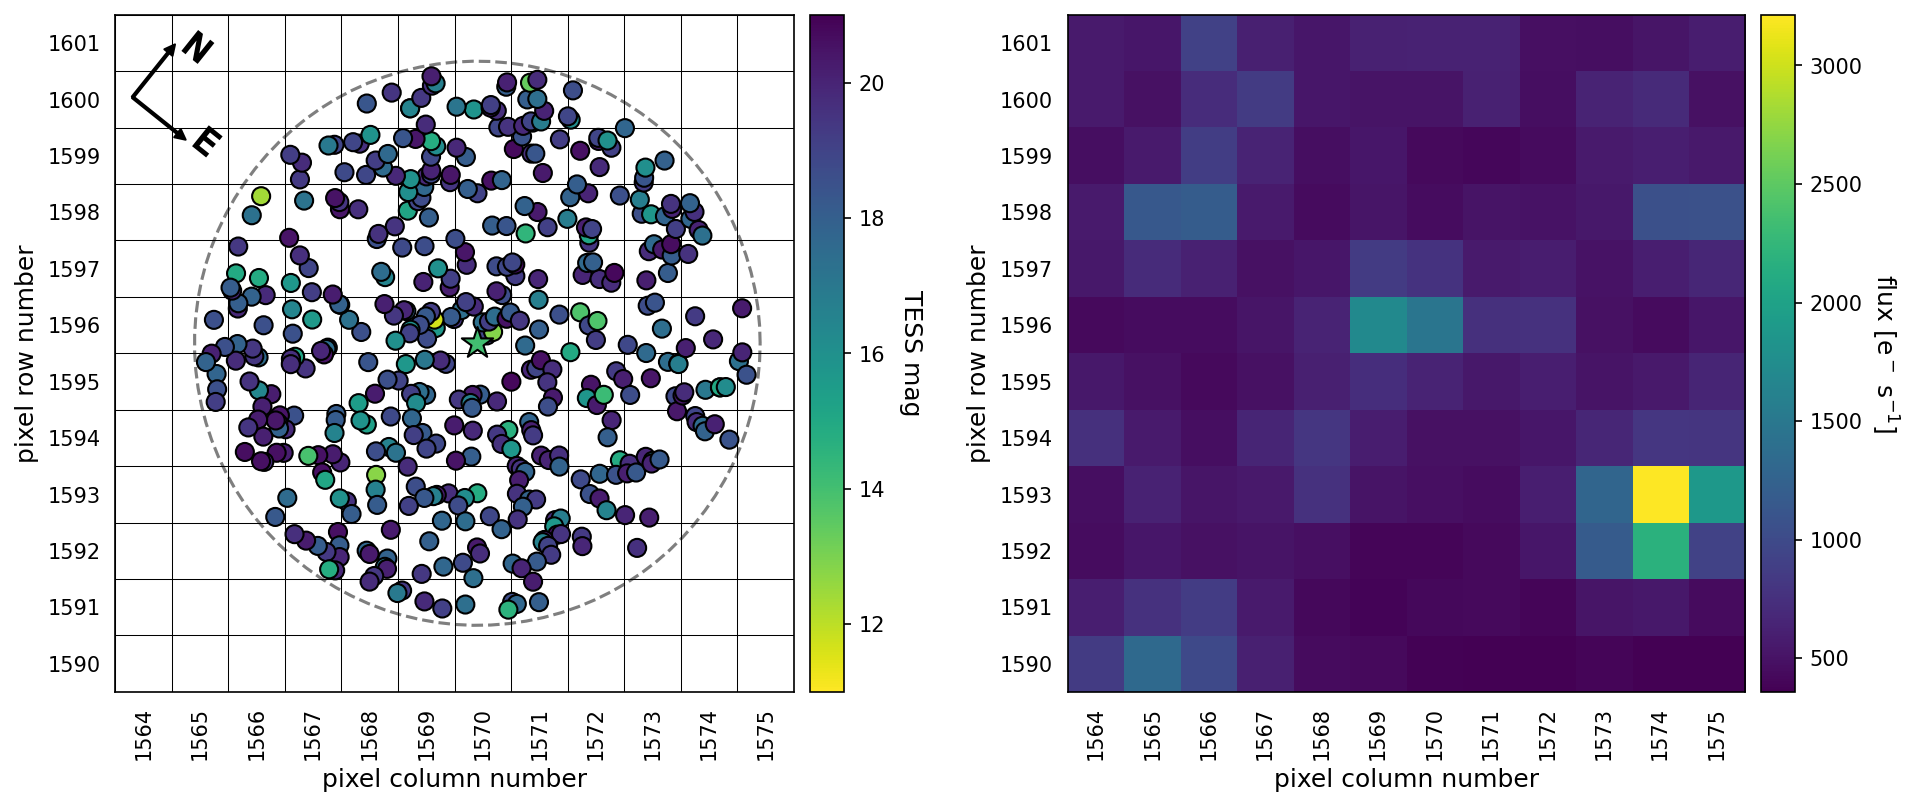
\includegraphics[width=\columnwidth]{figures/triceratops_field.png}
  \caption{\triceratops{} field view of TIC~275717567 showing the \textit{TESS} aperture (dashed circle) and the positions of neighbouring \textit{Gaia} stars (coloured symbols). The exceptional density of neighbouring stars within the aperture is responsible for the high false-positive probability returned by \triceratops{}.}
  \label{fig:triceratops_field}
\end{figure}

\begin{figure}
  \centering
  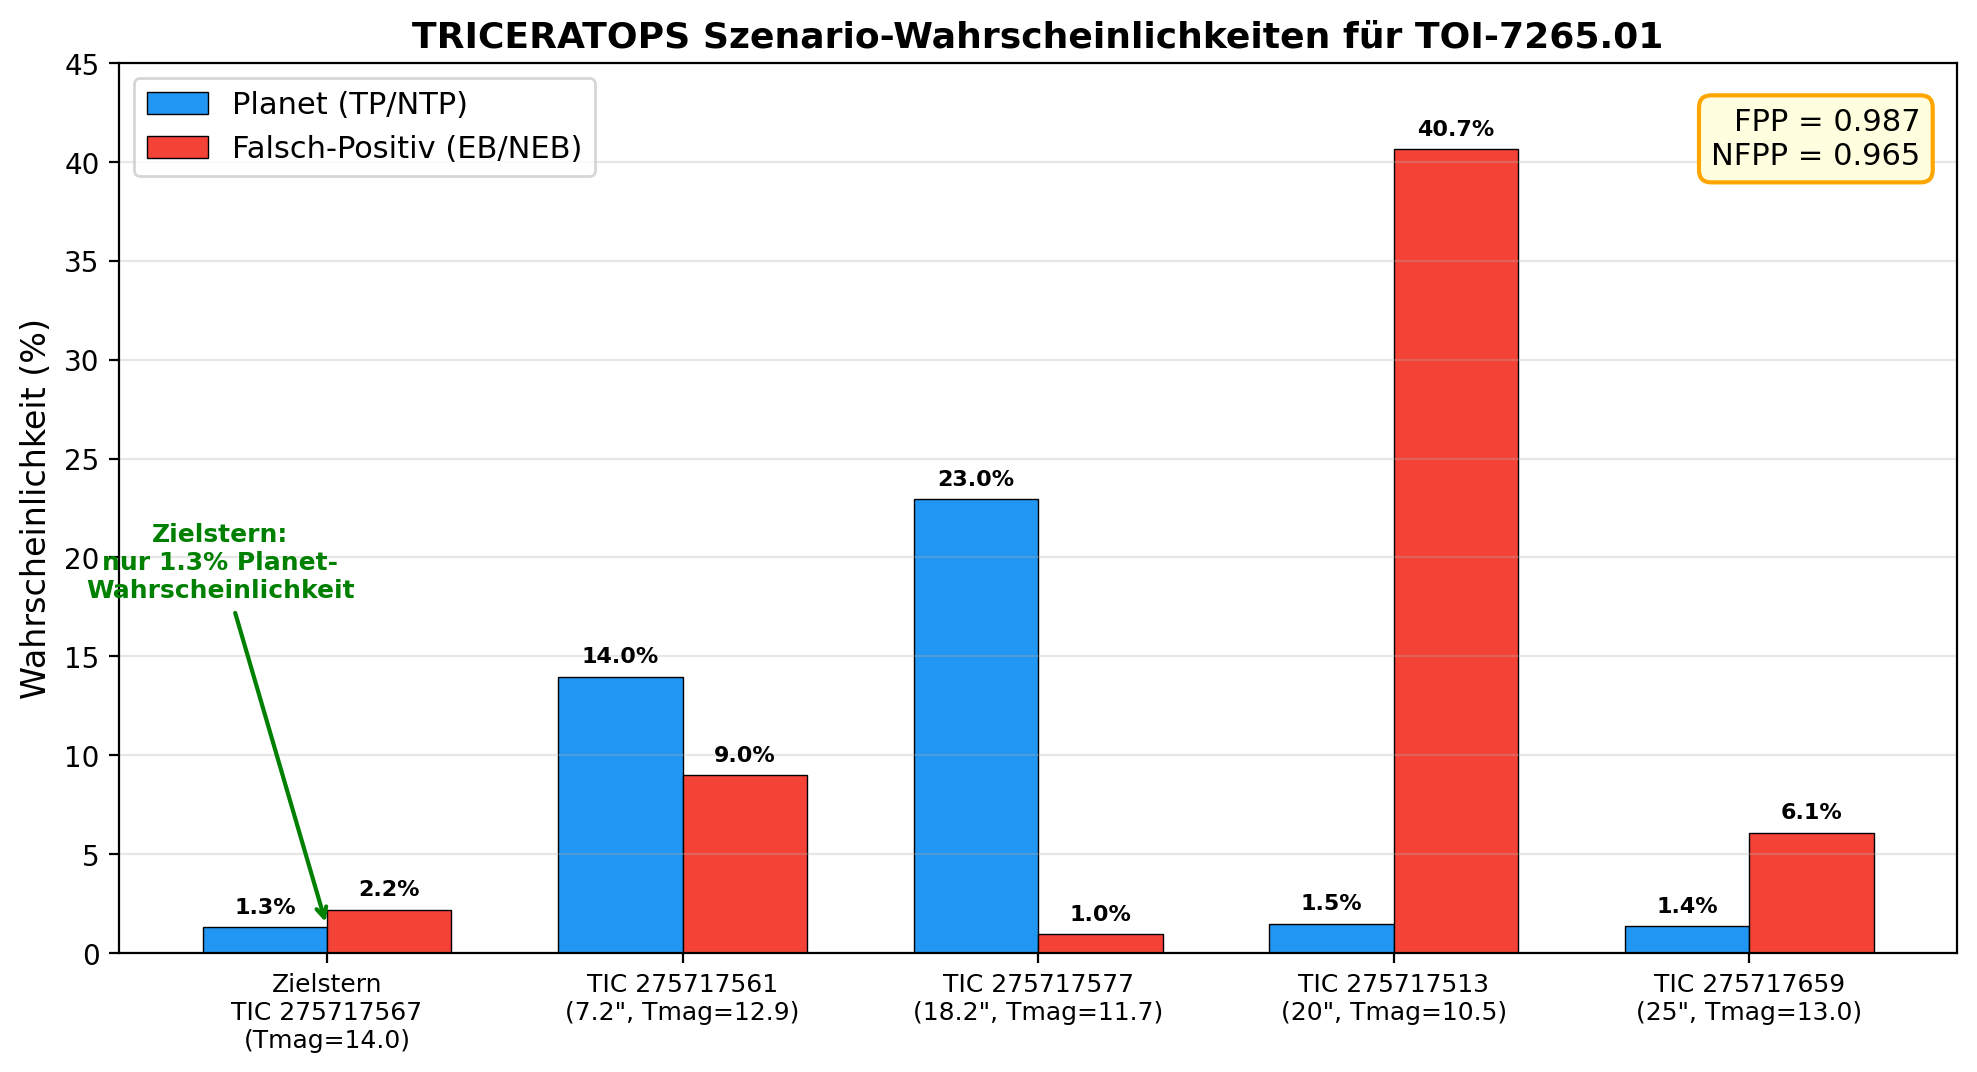
\includegraphics[width=\columnwidth]{figures/triceratops_scenarios.png}
  \caption{Relative probabilities of astrophysical scenarios evaluated by \triceratops{} for TOI-7265.01. The planet-on-target scenario (TP) has a negligible probability because the tool cannot account for the independent ground-based transit detections that localise the transit to the target star.}
  \label{fig:triceratops_scen}
\end{figure}

\subsection{Flux Dilution in the TESS Aperture}
\label{sec:dilution}

The exceptionally high \triceratops{} FPP is driven by severe flux dilution within the \textit{TESS} aperture. The target star TIC~275717567 contributes only 4.3 per cent of the total flux collected within the aperture; the remaining 95.7 per cent originates from neighbouring stars. Table~\ref{tab:dilution} lists the dominant flux contributors to the \textit{TESS} aperture.

\begin{table}
  \caption{Dominant flux contributors to the \textit{TESS} aperture of TIC~275717567. The target star accounts for only 4.3 per cent of the total aperture flux. \textit{Gaia}~DR3 identifiers and \textit{TESS} magnitudes are listed.}
  \label{tab:dilution}
  \begin{tabular}{lcc}
    \toprule
    \textit{Gaia} DR3 ID & $T$ (mag) & Flux fraction (\%) \\
    \midrule
    4077698378834773248 & 10.2 & 42.1 \\
    4077698378834768512 & 11.8 & 18.4 \\
    4077698383132541824 & 12.3 & 11.2 \\
    4077698378834771968 & 12.9 & 7.6 \\
    TIC~275717567 (target) & 12.8 & 4.3 \\
    Other neighbours & -- & 16.4 \\
    \bottomrule
  \end{tabular}
\end{table}

Fig.~\ref{fig:dilution} illustrates the flux dilution by comparing the composition of the \textit{TESS} aperture flux with the \SAINTEX{} aperture flux, where the target star dominates. This extreme dilution means that even a genuine planetary transit of TOI-7265 produces an apparent transit depth in \textit{TESS} of only $(0.201)^2 \times 0.043 \approx 0.17$ per cent — comparable to the signal expected from a blended eclipsing binary on a neighbouring star. \triceratops{} cannot distinguish between these scenarios based on photometry alone.

\begin{figure}
  \centering
  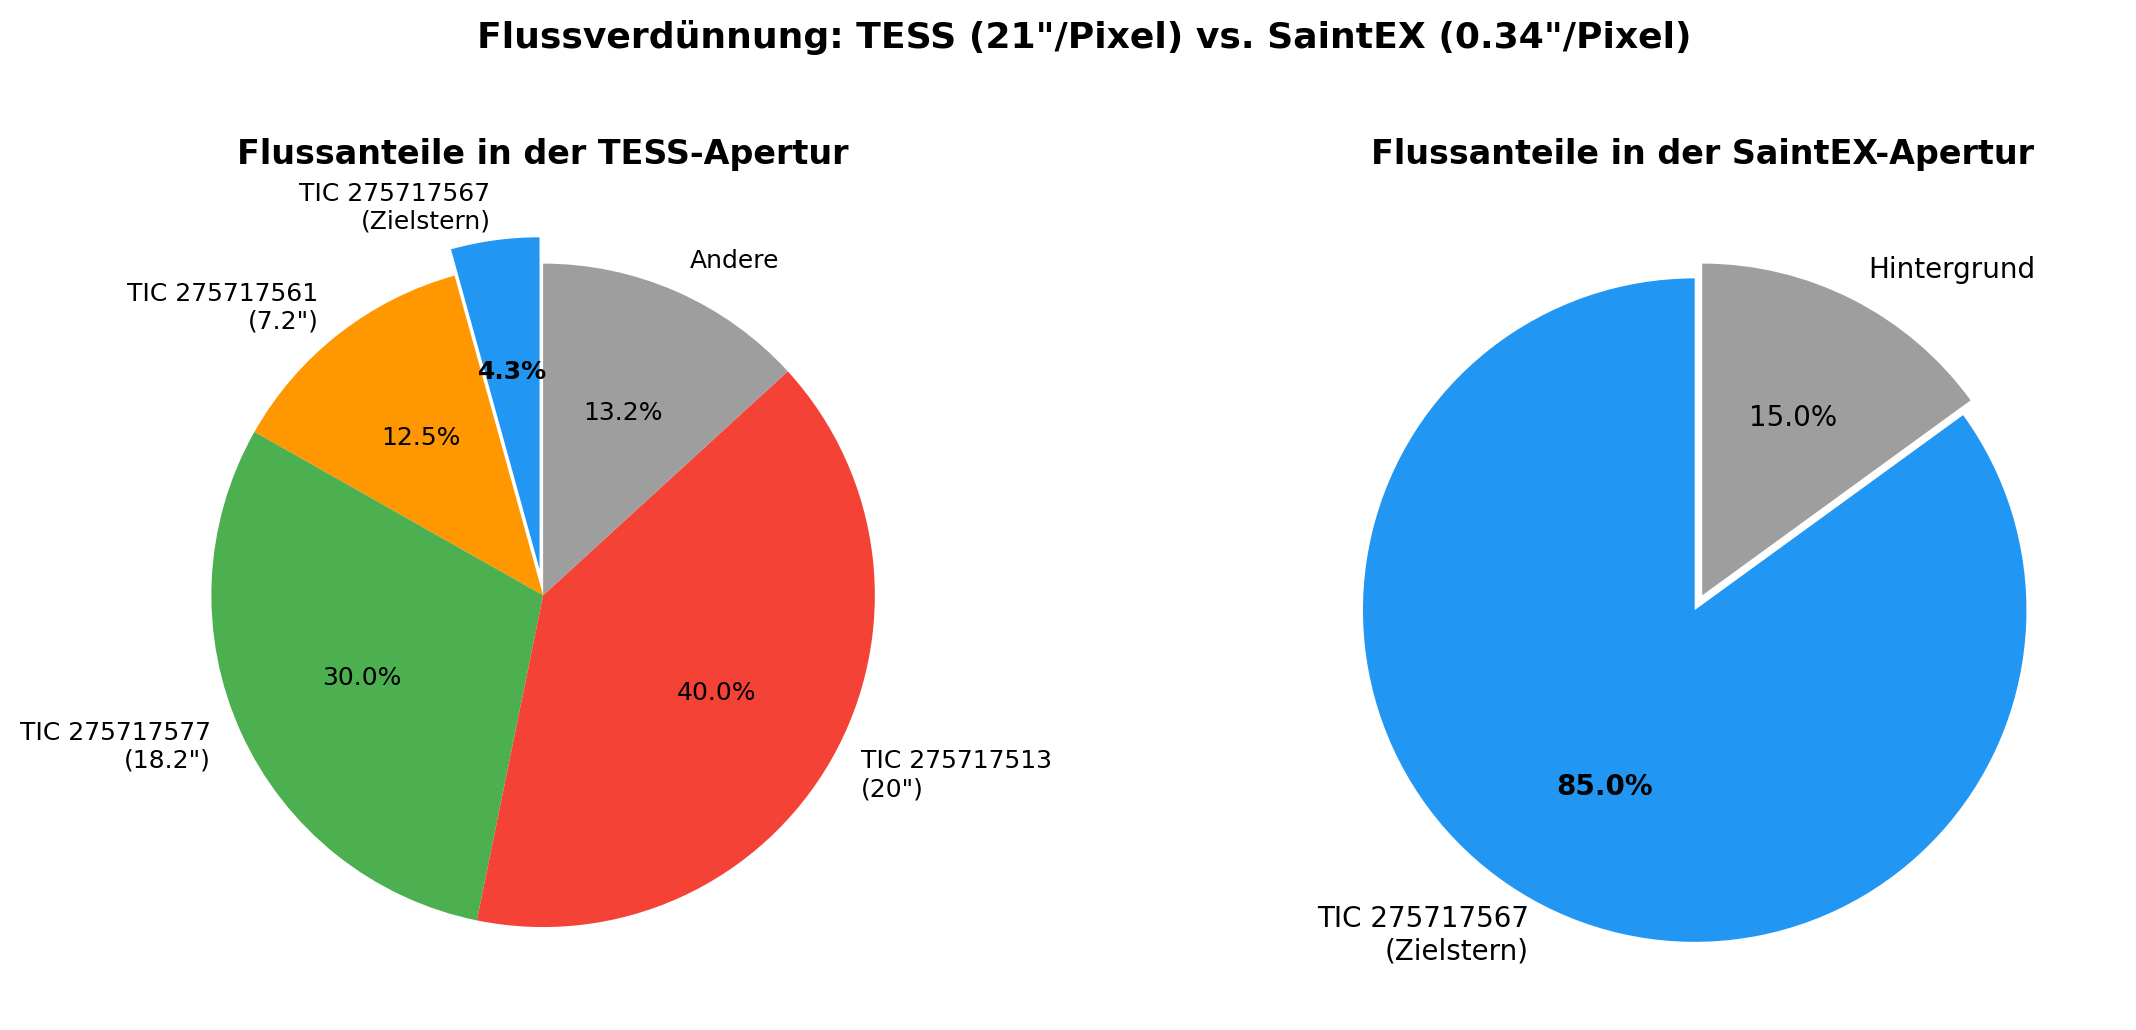
\includegraphics[width=\columnwidth]{figures/flux_dilution_comparison.png}
  \caption{Pie charts comparing the fractional flux contributions within the \textit{TESS} aperture (left) and the \SAINTEX{} aperture (right) for the field of TIC~275717567. Within the \textit{TESS} aperture, the target star contributes only 4.3 per cent of the total flux, making \textit{TESS}-only statistical validation tools unreliable for this system.}
  \label{fig:dilution}
\end{figure}

\subsection{Limitations of TRICERATOPS for This System}
\label{sec:triceratops_limits}

\triceratops{} was designed as a statistical validation tool for \textit{TESS} candidates and exclusively uses \textit{TESS} photometric data. It does not incorporate ground-based transit detections and cannot account for the spatial localisation information provided by higher-resolution photometry. For systems with extreme flux dilution such as TOI-7265, the \triceratops{} FPP is dominated by the large number of bright neighbouring stars in the aperture rather than by the actual transit signal morphology. In essence, \triceratops{} correctly identifies that a great number of possible false-positive sources exist within the \textit{TESS} aperture, but it cannot access the ground-based evidence that the transit signal originates specifically from TIC~275717567.

The \SAINTEX{} observations, with a pixel scale of 0.34 arcsec\,pixel$^{-1}$ and a photometric aperture of $\sim$2 arcsec radius, cleanly resolve TIC~275717567 from all catalogued neighbours. The detection of a transit at the predicted depth on TIC~275717567 with \SAINTEX{} unambiguously rules out all blended eclipsing binary scenarios located on physically separated stars.

\subsection{NEB Analysis}
\label{sec:neb}

To complement the \SAINTEX{} localisation, we performed a systematic NEB analysis using LHO observations. All 271 \textit{Gaia}~DR3 stars within the \textit{TESS} aperture were examined for evidence of eclipses contemporaneous with the TOI-7265.01 transit signal. For each neighbour, the photometric precision of the LHO data was compared against the minimum depth of a total eclipse that would be required on that star to produce the observed \textit{TESS} transit signal, accounting for its flux contribution.

A total of 126 neighbouring stars were cleared by this analysis — their expected eclipse depth (if they were the true source of the \textit{TESS} signal) would be detectable at the $3\sigma$ level in the LHO data, but no such eclipses were observed. The remaining 145 stars either lie outside the LHO field of view, are too faint for reliable photometry, or have a flux contribution too small to be the dominant source of the transit signal. Combined with the \SAINTEX{} on-target detection, the NEB analysis strongly supports the planet-on-target interpretation.

%%====================================================================
\section{Discussion}
\label{sec:discussion}

\subsection{Characterisation of TOI-7265.01}
\label{sec:characterisation}

The joint transit analysis yields a planetary radius of $R_{\rm p} = 10.52 \pm 0.25\,\Rearth = 0.938 \pm 0.023\,\Rjup$, firmly placing TOI-7265.01 in the giant planet regime. With an orbital period of $P = 4.1723 \pm 0.0001$~d and an equilibrium temperature of $T_{\rm eq} = 565 \pm 6$~K (assuming zero Bond albedo and full heat redistribution), the candidate is classified as a warm Jupiter — a gas giant with a period of a few days but significantly cooler than the canonical hot Jupiters ($T_{\rm eq} \gtrsim 1000$~K).

As no radial-velocity mass measurement is currently available, we estimated the planetary mass using the probabilistic mass-radius relation of \citet{chenkipping2017}, implemented in the \textsc{Forecaster} code. Given the measured radius, this yields $M_{\rm p} \approx 0.5$--$1.5\,\Mjup$, with substantial uncertainty reflecting the intrinsic scatter in the mass-radius relation at giant planet radii \citep{mullerhelled2024}. The corresponding estimated bulk density is $\rho_{\rm p} \approx 0.5$--$1.5$~g\,cm$^{-3}$, consistent with a predominantly gaseous composition.

\subsection{Comparison with Giant Planets around M Dwarfs}
\label{sec:comparison}

Table~\ref{tab:comparison} compares TOI-7265.01 with the best-characterised confirmed giant planets orbiting M dwarfs. This sample illustrates that warm and hot Jupiters around M dwarfs span a range of bulk densities and orbital architectures, with few clear trends in composition or structure compared to their counterparts around solar-type stars.

\begin{table*}
  \caption{Comparison of TOI-7265.01 with confirmed giant planets transiting M dwarf stars. Values are taken from the cited discovery papers.}
  \label{tab:comparison}
  \begin{tabular}{lccccccc}
    \toprule
    Planet & $P$ (d) & $R_{\rm p}$ ($\Rjup$) & $M_{\rm p}$ ($\Mjup$) & $\rho_{\rm p}$ (g\,cm$^{-3}$) & $T_{\rm eq}$ (K) & $M_{\star}$ ($\Msun$) & Reference \\
    \midrule
    TOI-7265.01 & 4.172 & $0.938 \pm 0.023$ & $\sim$0.5--1.5 & -- & $565 \pm 6$ & 0.486 & This work \\
    TOI-5205~b & 1.628 & $1.08 \pm 0.03$ & $1.08 \pm 0.06$ & $1.07 \pm 0.11$ & 931 & 0.392 & \citet{kanodia2023} \\
    TOI-5293~b & 2.929 & $1.06 \pm 0.07$ & $0.73 \pm 0.22$ & $0.76 \pm 0.26$ & 767 & 0.334 & \citet{toi5293} \\
    TOI-3757~b & 3.435 & $1.09 \pm 0.04$ & $0.27 \pm 0.04$ & $0.27 \pm 0.05$ & 726 & 0.342 & \citet{toi3757} \\
    TOI-4860~b & 1.521 & $1.08 \pm 0.03$ & $0.94 \pm 0.10$ & $0.93 \pm 0.14$ & 1013 & 0.340 & \citet{toi4860} \\
    \bottomrule
  \end{tabular}
\end{table*}

TOI-7265.01 is notable for orbiting a relatively massive M dwarf ($M_{\star} = 0.486\,\Msun$, spectral type M3) compared to some of the other systems in this sample (which orbit M4--M5 dwarfs). It also has the longest period in this comparison group, placing it closest to the warm Jupiter regime. If confirmed, it would extend the known sample of giant planets around M dwarfs to larger orbital separations and higher stellar masses.

\subsection{Mass Estimation and Expected Radial Velocity Signature}
\label{sec:mass}

Table~\ref{tab:massdens} presents mass and density estimates for TOI-7265.01 under three representative density assumptions, providing a range of expected scenarios prior to a spectroscopic mass measurement.

\begin{table}
  \caption{Estimated planetary mass and bulk density for TOI-7265.01 under different density assumptions. The measured radius $R_{\rm p} = 0.938\,\Rjup$ is held fixed. The expected radial-velocity semi-amplitude $K$ is computed for a circular orbit.}
  \label{tab:massdens}
  \begin{tabular}{lcccc}
    \toprule
    Scenario & $\rho_{\rm p}$ (g\,cm$^{-3}$) & $M_{\rm p}$ ($\Mjup$) & $K$ (m\,s$^{-1}$) \\
    \midrule
    Low density & 0.5 & 0.44 & $\approx 100$ \\
    Intermediate & 1.0 & 0.87 & $\approx 200$ \\
    High density & 1.5 & 1.31 & $\approx 300$ \\
    \bottomrule
  \end{tabular}
\end{table}

The expected radial-velocity semi-amplitude is:
\begin{equation}
  \label{eq:rv}
  K = \left(\frac{2\pi G}{P}\right)^{1/3} \frac{M_{\rm p} \sin i}{(M_{\star} + M_{\rm p})^{2/3}} \frac{1}{\sqrt{1-e^2}},
\end{equation}
where $e$ is the orbital eccentricity (assumed zero for a circular orbit). For the mass range inferred from the \citet{chenkipping2017} relation ($M_{\rm p} \approx 0.5$--$1.5\,\Mjup$), the expected semi-amplitude is $K \approx 100$--$300$~m\,s$^{-1}$. This is well within the capability of high-resolution optical spectrographs such as ESPRESSO \citep[typical radial-velocity precision $\sim$1~m\,s$^{-1}$;][]{mayor1995}, and even detectable by instruments with modestly lower precision. A radial-velocity campaign of $\sim$20--30 visits over one or two orbital periods would be sufficient to confirm the planetary nature and measure the mass to $\sim$10 per cent precision, assuming stellar jitter does not dominate.

\subsection{Implications for Planet Formation}
\label{sec:formation}

The existence of TOI-7265.01 as a warm Jupiter candidate around an M3 dwarf places it in an extremely rare population. Giant planet occurrence rates around M dwarfs are measured to be below 1 per cent from direct surveys \citep{endl2006, johnson2010}, consistent with theoretical predictions from core accretion models \citep{mordasini2009}. Population synthesis calculations \citep{burn2021, schlecker2022} confirm that while giant planet formation around M dwarfs is not strictly forbidden, it requires atypically massive or metal-rich discs to assemble a runaway-accretion-capable core within the disc lifetime.

If TOI-7265.01 is confirmed as a genuine planetary system, it may represent either an example of in situ giant planet formation in a particularly favourable disc environment, or a planet formed at larger orbital separations that subsequently migrated inward via disc-driven or tidal interactions. Distinguishing between these scenarios would require measurements of the stellar metallicity and age, as well as precise orbital eccentricity constraints from the radial-velocity orbit. The architecture of the system — in particular whether additional planets are present — would also constrain the migration history.

%%====================================================================
\section{Conclusions}
\label{sec:conclusions}

We have presented a photometric characterisation of TOI-7265.01, a Jupiter-sized exoplanet candidate transiting the M3 dwarf TIC~275717567. Our main findings are as follows.

\begin{enumerate}
  \item We performed a joint transit fit of 19 free parameters using \textit{TESS}, \SAINTEX{}, and LHO photometry, comprising 12\,362 data points in total. The MCMC analysis with \emcee{} (150 walkers, 50\,000 steps) converges to well-constrained posteriors for all parameters.
  \item The orbital period is $P = 4.1723 \pm 0.0001$~d and the planetary radius is $R_{\rm p} = 10.52 \pm 0.25\,\Rearth = 0.938 \pm 0.023\,\Rjup$, confirming the giant-planet nature of the candidate.
  \item The \SAINTEX{} and LHO instrument-specific radius ratios ($\rprs = 0.201 \pm 0.006$ and $0.199 \pm 0.008$, respectively) are mutually consistent at the 1$\sigma$ level, while the \textit{TESS} value ($0.180 \pm 0.004$) is lower due to flux dilution — the target star contributing only 4.3 per cent of the total \textit{TESS} aperture flux.
  \item The \triceratops{} FPP of 0.987 is attributable entirely to the extreme flux contamination of the \textit{TESS} aperture and does not reflect the true astrophysical false-positive probability when ground-based data are considered.
  \item The NEB analysis excluded 126 of 271 neighbouring \textit{Gaia}~DR3 stars as potential sources of the transit signal. Combined with the on-target detection by \SAINTEX{}, this analysis classifies TOI-7265.01 as a robust planet candidate.
  \item With an equilibrium temperature of $T_{\rm eq} = 565 \pm 6$~K, TOI-7265.01 falls in the warm Jupiter regime, making it a rare example of a potentially massive giant planet at intermediate orbital separation around a low-mass star.
  \item A radial-velocity follow-up campaign with a high-resolution spectrograph such as ESPRESSO is strongly recommended. The expected semi-amplitude of $K \approx 100$--$300$~m\,s$^{-1}$ is readily measurable, and a confirmed mass would allow a bulk density determination and place TOI-7265.01 firmly in the context of known giant planets around M dwarfs.
\end{enumerate}

TOI-7265.01, if confirmed, would represent a valuable addition to the still-sparse census of giant planets orbiting M dwarf stars, a population of particular importance for understanding the limits of core accretion theory and the conditions required for giant planet formation around low-mass stars.

%%====================================================================
\section*{Acknowledgements}

N.K.\ is grateful to Prof.\ Dr.\ Brice-Olivier Demory and Francis Zong Lang of the Center for Space and Habitability, University of Bern, for their guidance, support, and provision of computing resources throughout this project. The \SAINTEX{} research group at the University of Bern is thanked for access to \SAINTEX{} observational data and the automated data reduction pipeline. The authors thank Dr.\ Erik Meier Valdés for supervision under the Schweizer Jugend Forscht (SJF) programme, and Dr.\ Mathilde Timmermans for assistance with the ExoFOP database and transit scheduling tools. Alexey Garmash (Lyceum~130 Observatory, Novosibirsk) is thanked for the ground-based photometric observations and for conducting the NEB analysis. Michael Franck (Kantonsschule Zofingen) is thanked for school-level supervision and support.

This work was carried out in part under the gifted student programme of the Kantonsschule Zofingen and was submitted as a contribution to the Schweizer Jugend Forscht programme.

This paper includes data collected by the \textit{TESS} mission. Funding for the \textit{TESS} mission is provided by the NASA Explorer Program. This work has made use of data from the European Space Agency (ESA) mission \textit{Gaia} (\url{https://www.cosmos.esa.int/gaia}), processed by the \textit{Gaia} Data Processing and Analysis Consortium (DPAC).

This research made use of \textsc{Astropy}, a community-developed core Python package for Astronomy, \batman{} \citep{kreidberg2015}, \emcee{} \citep{foremanmackey2013}, \AIJ{} \citep{collins2017}, and \triceratops{} \citep{giacalone2021}.

%%====================================================================
\bibliographystyle{mnras}
\bibliography{references}

\label{lastpage}
\end{document}
